%  Μεταγλώττιση με XeLaTeX

\documentclass{llncs}
\pagestyle{headings} 
%
\usepackage{makeidx}  % allows for indexgeneration
%
\usepackage{xltxtra}
\usepackage{xgreek}

\usepackage{caption}
\usepackage{subcaption}

\setsansfont{Arial}
\setmonofont{Courier New}
\setmainfont[Mapping=tex-text]{Times New Roman}
% \setmainfont[Mapping=tex-text]{GFS Didot} 
% \setsansfont{GFS Didot}
% \setmonofont{GFS Didot}

\renewcommand{\abstractname}{Περίληψη}
\newtheorem{observation}{Παρατήρηση}
\renewcommand{\keywordname}{\bf Λέξεις Κλειδιά:}
\renewcommand\refname{Αναφορές}
\renewcommand\ackname{Ευχαριστίες}
\renewcommand\andname{και}
\renewcommand\corollaryname{Πόρισμα}
\renewcommand\definitionname{Ορισμός}
\renewcommand\examplename{Παράδειγμα}
\renewcommand\exercisename{Άσκηση}
\renewcommand\figurename{Εικ.}
\renewcommand\lemmaname{Λήμμα}
\renewcommand\proofname{Απόδειξη}
\renewcommand\propositionname{Πρόταση}
\renewcommand\solutionname{Λύση}
\renewcommand\tablename{Πίνακας}
\renewcommand\theoremname{Θεώρημα}

\begin{document}
%
\title{\Huge Προγραμματιστική Εργασία Πρόβλεψη κόστους ασφάλισης οχημάτων}
%
%
\author{\Large Χαρά Τσίρκα \and Πρόδρομος Αβραμίδης \and Γεώργιος Γεροντίδης}
%
%
%
\institute{\email{\{ctsirka, pavramidis, ggerontidis\}@e-ce.uth.gr}\\
8$^{ο}$ εξάμηνο\\
\begin{center}
    \vspace{1cm}
    
\includegraphics[width=0.4\textwidth]{uthlogo.png}
    \vspace{1cm}
\end{center}
\Large Τμήμα Ηλεκτρολόγων Μηχανικών \& Μηχανικών Υπολογιστών\\
Πανεπιστήμιο Θεσσαλίας, Βόλος\\
\vspace{1cm}
{\bf \Large Εξόρυξη Δεδομένων 2023-24}\\
\Large Διδάσκον: Μ.Βασιλακόπουλος\\
\vspace{1cm}
Μάιος 2024}

\maketitle


\section{Εισαγωγή}
Η εργασία μας επικεντρώνεται στην πρόβλεψη του κόστους ασφάλισης μηχανοκίνητων οχημάτων. Η ανάλυση αυτή αποτελεί ένα κρίσιμο ζήτημα στον τομέα της ασφάλισης, 
καθώς επιτρέπει στους ασφαλιστές να προσδιορίζουν με μεγαλύτερη ακρίβεια τα ασφαλιστικά ασφάλιστρα, λαμβάνοντας υπόψη διάφορους παράγοντες που επηρεάζουν το κόστος.
Η διαδικασία της εργασίας ξεκινά με την προ-επεξεργασία των δεδομένων, κατά την οποία πραγματοποιήθηκε εξερευνητική ανάλυση (exploratory analysis) για τον προσδιορισμό 
των κριτηρίων διαχωρισμού των δεδομένων. Κατά τη διάρκεια αυτής της ανάλυσης, μετρήθηκε ο βαθμός επίδρασης κάθε χαρακτηριστικού (feature) του συνόλου δεδομένων στα αποτελέσματα. 
Με τη βοήθεια διαγραμμάτων, καταφέραμε να επιλέξουμε τον κατάλληλο διαχωρισμό των δεδομένων για περαιτέρω ανάλυση. Στη συνέχεια, η εργασία θα προχωρήσει στη δημιουργία και 
αξιολόγηση των μοντέλων πρόβλεψης, λαμβάνοντας υπόψη την είσοδο των χρηστών, ενώ θα ακολουθήσει η οπτικοποίηση και η αξιολόγηση των αποτελεσμάτων.

\section{Περιγραφή dataset}
Το dataset το οποίο επιλέξαμε αποτελείται από 30 μεταβλητές (columns) και 105555 εγγραφές. Στους παρακάτω πίνακες δίνεται μία σύντομη περιγραφή της κάθε μεταβλητής:

\begin{center}
    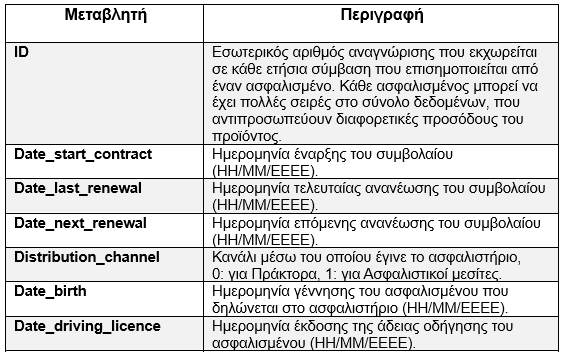
\includegraphics[width=1\textwidth]{images/variables_1.png}
\end{center}

\begin{center}
    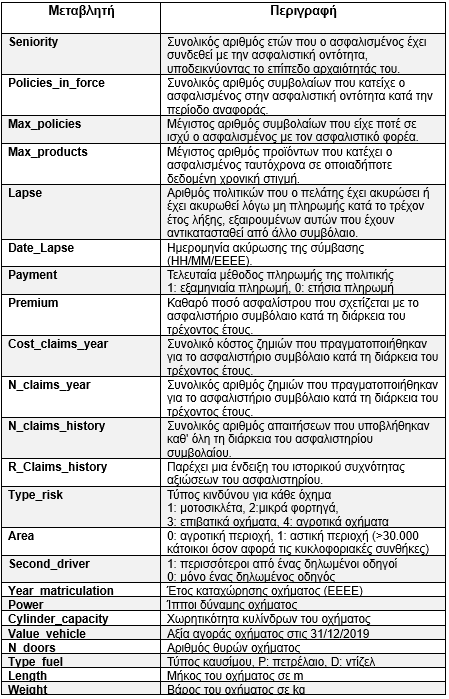
\includegraphics[width=1\textwidth]{images/variables_2.png}
\end{center}

\newpage
\section{Data preproccesing}
Το πρώτο βήμα για την προεπεξεργασία των δεδομένων ήταν να κρατήσουμε μία γραμμή για κάθε 'ID'. Σε ένα 'ID' μπορεί να αντιστοιχούν  περισσότερες από μία γραμμές που αντιπροσωπεύουν το 
ίδιο συμβόλαιο του ίδιου πελάτη για διαφορετική χρονική περίοδο. Έτσι, για κάθε 'ID' κρατάμε την τελευταία ανανέωση του συμβολαίου, δηλαδή την γραμμή με το μεγαλύτερο χρονολογικά 'last\_renewal\_date'. 
Έπειτα, στη θέση του 'premium' υπολογίζουμε και τοποθετούμε τον μέσο όρο των 'premium' όλων των γραμμών με κοινό 'ID'.

Το δεύτερο βήμα ήταν η επεξεργασία όλων των ημερομηνιών. Ειδικότερα, οι στήλες 'Date\_birth', 'Date\_driving\_license', 'Date\_start\_contract', 'Date\_last\_renewal', \\
'Date\_next\_renewal', 'Date\_lapse' δίνονται στην μορφή ΗΗ/ΜΜ/ΕΕΕΕ. Αρχικά, για κάθε μία από αυτές τις μεταβλητές κρατήσαμε το έτος (ΕΕΕΕ) και στην συνέχεια πραγματοποιώντας τις κατάλληλες αφαιρέσεις
δημιουργήσαμε νέες στήλες στο dataset που πήραν την θέση αυτών που αναφέρθηκαν νωρίτερα. Έτσι, δημιουργήσαμε τις στήλες: 'Age' που προσδιορίζει την ηλικία του πελάτη, 'Years\_driving' που προσδιορίζει 
πόσα χρόνια οδηγεί ο πελάτης, 'Year\_on\_road' που προσδιορίζει πόσα χρόνια κυκλοφορεί το κάθε όχημα υπό την κατοχή συγκεκριμένου πελάτη, 'Policy Duration' που υποδεικνύει την διάρκεια του εκάστοτε συμβολαίου σε χρόνια και 
'Years\_on\_policy' που προσδιορίζει πόσα χρόνια ο πελάτης βρίσκεται στον ίδιο τύπο συμβολαίου. Πρέπει να σημειωθεί πως το dataset περιέχει δεδομένα μέχρι και το 2019. Για να έχουμε μια σωστή εικόνα των χρονολογιών
σε όλες αυτές τις μεταβλητές που δημιουργήσαμε, χρησιμοποιήσαμε ως σημείο αναφοράς την χρονολογία τελευταίας ανανέωσης του συμβολαίου. Για παράδειγμα η μεταβλητή 'Age' προκύπτει από την αφαίρεση:
'Age' = 'Date\_last\_renewal' - 'Date\_birth'.

Επιπλέον, δημιουργήσαμε μία ακόμη νέα στήλη με όνομα 'accidents' για να υπάρχει μια συσχέτιση μεταξύ των αριθμών των ατυχημάτων με τα χρόνια που ένας πελάτης είναι ασφαλισμένος στην εταιρεία.

Διαχειριστήκαμε την απουσία τιμών με δύο τρόπους. Στην στήλη 'Length' αντικαταστήσαμε τα κενά πεδία με τον μέσο όρο των τιμών της στήλης. Στην στήλη 'Type\_fuel' αντικαταστήσαμε τα κενά πεδία με την τιμή 
'Unknown'.

Μετά από δοκιμές διαπιστώσαμε πως κάποιες μεταβλητές του dataset δεν συνεισέφεραν καθόλου στην βελτίωση της απόδοσης και παραλείφθηκαν. Οι στήλες που χρησιμοποιήθηκαν τελικά είναι οι: 
'Seniority', 'Premium', 'Type\_risk', 'Area', 'Power', 'Second\_driver', 'Years\_on\_road', 'R\_claims\_history', 'Years\_on\_policy', 'accidents', 'Value\_vehicle, 'Age', 'Years\_driving', 'Distribution\_channel', 'N\_claims\_history',
\\ 'Cylinder\_capacity', 'Weight', 'Length', 'Type\_fuel', 'Payment', 'Contract\_year', \\'Policies\_in\_force', 'Lapse'.



\section{Εκπαίδευση μοντέλου}


\noindent \textbf{XGBoost Parameters}

(Στις παρενθέσεις βρίσκεται το συνηθισμένο εύρος τιμών, δηλαδή το εύρος που έγιναν οι δοκιμές για να πετύχουμε το μέγιστο επιθυμητό αποτέλεσμα.)

\noindent \textbf{Objective (linear):}

Το `reg:squarederror` είναι το προεπιλεγμένο και ευρέως χρησιμοποιούμενο loss function για regression tasks, παρέχοντας ένα σαφές πλαίσιο για τη βελτιστοποίηση του μοντέλου XGBoost. Συγκεκριμένα, είναι κατάλληλο για την πρόβλεψη ασφάλιστρων, καθώς στοχεύει στην επίτευξη υψηλής ακρίβειας στην πρόβλεψη της συνεχούς τιμής των ασφάλιστρων.

\noindent \textbf{Eval\_metric (`rmse`, `mae`):}

Για το eval\_metric, επιλέξαμε το `rmse` (Root Mean Squared Error) επειδή είναι ένα ευρέως αποδεκτό μέτρο για regression tasks. Αναλυτικότερα, δίνει μεγαλύτερη βαρύτητα σε μεγαλύτερες αποκλίσεις (λάθη) μεταξύ πραγματικών και προβλεπόμενων τιμών, γεγονός που μπορεί να είναι χρήσιμο στην ασφαλιστική πρόβλεψη όπου τα μεγάλα λάθη μπορεί να είναι πιο σοβαρά.

\noindent \textbf{Learning\_rate (0.001-0.3):}

Ο ρυθμός μάθησης (learning rate) επηρεάζει πόσο γρήγορα προσαρμόζεται το μοντέλο κατά την εκπαίδευση. Επιλέχθηκε η τιμή 0.01 έπειτα από δοκιμές, διότι όντας χαμηλή σχετικά τιμή επιβραδύνει τη διαδικασία μάθησης, μειώνοντας την πιθανότητα υπερβολικής προσαρμογής (overfitting).

\noindent \textbf{Max\_depth (3-10):}

Το μέγιστο βάθος των δέντρων στο μοντέλο. Ένας μεγαλύτερος αριθμός επιτρέπει πιο περίπλοκα δέντρα, αλλά μπορεί να οδηγήσει σε overfitting, επομένως επιλέχθηκε η τιμή 6.

\noindent \textbf{Min\_child\_weight (1-10):}

Ελάχιστο βάρος που πρέπει να έχει ένας κόμβος για να διαχωριστεί. Επηρεάζει την ευαισθησία του μοντέλου στις διακυμάνσεις στα δεδομένα. Ύστερα από δοκιμές προτιμήθηκε ο αριθμός βάρους 5.

\noindent \textbf{Subsample (0.5-1):}

Αναφέρεται στο ποσοστό των δειγμάτων που θα χρησιμοποιηθούν σε κάθε επανάληψη της εκπαίδευσης. Ένα ποσοστό 0.8 σημαίνει ότι το 80% των δειγμάτων θα χρησιμοποιηθεί.

\noindent \textbf{Colsample\_bytree (0.5-1):}

Το ποσοστό των χαρακτηριστικών (columns) που θα επιλεχθούν τυχαία για να κατασκευάσουν κάθε δέντρο στο μοντέλο. Ένα ποσοστό 0.8 σημαίνει ότι το 80% των χαρακτηριστικών θα χρησιμοποιηθεί σε κάθε δέντρο.

\noindent \textbf{N\_estimators (100-2000):}

Ο αριθμός των δέντρων που θα κατασκευαστούν στο μοντέλο. Δοκιμάστηκαν διάφοροι αριθμοί, συμπεριλαμβανομένων μεγαλύτερων από 1000, αλλά δεν υπήρχε μεγάλη βελτίωση στην απόδοση του μοντέλου, ενώ ο χρόνος εκπαίδευσης αυξανόταν σημαντικά. Έτσι, ως optimal θεωρήθηκε η τιμή 1000.

\noindent \textbf{Seed:}

Για να καταφέρουμε να εξασφαλίσουμε επαναληψιμότητα στα δεδομένα μας και να αφαιρεθεί η τυχαιότητα, επιλέξαμε έναν σταθερό αριθμό seed 42.

\noindent \textbf{Random forest parameters:}


\noindent \textbf{N\_estimators (100-1000):}

Επιλέχθηκε η τιμή 700, διότι παρατηρήθηκε ότι, παρόλο που η αύξηση της τιμής βελτίωνε την απόδοση του RF, ο χρόνος εκτέλεσης αυξανόταν σημαντικά λόγω της δημιουργίας πολλών δέντρων.

\noindent \textbf{Max\_depth (10-20):}

Επιλέχθηκε η τιμή 15, καθώς η αύξηση της τιμής αυξάνει τον κίνδυνο overfitting, αν και προσφέρει σημαντική βελτίωση στην απόδοση του RF.

\noindent \textbf{Min\_samples\_split (2-10):}

Επιλέχθηκε η τιμή 4, που βρίσκεται στη μέση του εύρους τιμών, για να ισορροπήσει μεταξύ της πρόληψης του overfitting και της διατήρησης της απόδοσης του μοντέλου.

\noindent \textbf{Min\_samples\_leaf (2-10):}

Επιλέχθηκε η τιμή 2, διότι παρατηρήθηκε ότι η αύξηση της τιμής αυτής παραμέτρου βελτίωνε μόνο την απόδοση στο type\_risk4, ενώ έπεφτε η συνολική απόδοση σε κάθε άλλο τύπο οχήματος.

\noindent \textbf{Max\_features (`sqrt`, `log2`, ή float 0.1-1):}

Συνήθως, σε αλγορίθμους RF προτιμάται η τιμή `sqrt`, και αυτή επιλέχθηκε και από εμάς για καλύτερη απόδοση.

\noindent \textbf{Bootstrap (True, False):}

Επιλέξαμε να έχουμε bootstrap, καθώς βελτιώνονται σημαντικά τα αποτελέσματα σε σύγκριση με την επιλογή της μη ύπαρξης bootstrap.

\noindent \textbf{N\_jobs (-1, 1, αριθμός πυρήνων):}

Με την επιλογή της τιμής -1, χρησιμοποιούμε όλους τους διαθέσιμους πυρήνες.

\noindent \textbf{Random\_state:}

Πρόκειται για τιμή τυχαιότητας όπως το seed στο XGBoost. Έχει επιλεγεί και εδώ η τιμή 42.

\begin{table}[ht]
    \centering
    \begin{tabular}{l|cc}
        \hline
        Parameter & Before Tuning & After Tuning \\
        \hline
        \texttt{objective} & \texttt{reg:squarederror} & \texttt{reg:squarederror} \\
        \texttt{eval\_metric} & \texttt{rmse} & \texttt{rmse} \\
        \texttt{learning\_rate} & 0.05 & 0.01 \\
        \texttt{max\_depth} & 4 & 5 \\
        \texttt{min\_child\_weight} & 1 & 5 \\
        \texttt{subsample} & 0.7 & 0.8 \\
        \texttt{colsample\_bytree} & 0.7 & 0.8 \\
        \texttt{n\_estimators} & 500 & 1000 \\
        \texttt{seed} & 42 & 42 \\
        \hline
    \end{tabular}
    \caption{XGBoost Parameter Settings Before and After Tuning}
\end{table}

\begin{table}[ht]
    \centering
    \begin{tabular}{lccc|ccc}
        \hline
        & \multicolumn{3}{c}{Before Tuning} & \multicolumn{3}{c}{After Tuning} \\
        \hline
        & Mean squared error & Average Absolute Error & R² Score & Mean squared error & Average Absolute Error & R² Score \\
        \hline
        Motorbikes & 2298.58 & 30.097 & 0.564 & 2228.745 & 29.779 & 0.5779 \\
        Vans & 8087.68 & 61.148 & 0.367 & 7846.43 & 60.345 & 0.386 \\
        Passenger Cars & 10776.074 & 69.165 & 0.378 & 10693.593 & 69.07 & 0.383 \\
        Agricultural Vehicles & 356.954 & 13.416 & -0.266 & 311.899 & 12.15 & -0.1068 \\
        \hline
    \end{tabular}
    \caption{XGBoost Parameter Tuning Results}
\end{table}

\begin{table}[ht]
    \centering
    \begin{tabular}{l|cc}
        \hline
        Parameter & Before Tuning & After Tuning \\
        \hline
        \texttt{n\_estimators} & 100 & 700 \\
        \texttt{max\_depth} & 10 & 15 \\
        \texttt{min\_samples\_split} & 2 & 4 \\
        \texttt{min\_samples\_leaf} & 2 & 2 \\
        \texttt{max\_features} & \texttt{log2} & \texttt{sqrt} \\
        \texttt{bootstrap} & \texttt{False} & \texttt{True} \\
        \texttt{n\_jobs} & \texttt{-1} & \texttt{-1} \\
        \texttt{random\_state} & \texttt{42} & \texttt{42} \\
        \hline
    \end{tabular}
    \caption{RandomForest Parameter Settings Before and After Tuning}
\end{table}

\begin{table}[ht]
    \centering
    \begin{tabular}{lccc|ccc}
        \hline
        & \multicolumn{3}{c}{Before Tuning} & \multicolumn{3}{c}{After Tuning} \\
        \hline
        & Mean squared error & Average Absolute Error & R² Score & Mean squared error & Average Absolute Error & R² Score \\
        \hline
        Motorbikes & 2380.952 & 30.542 & 0.549 & 2265.092 & 29.42 & 0.571 \\
        Vans & 8345.571 & 62.057 & 0.3476 & 8184.899 & 61.395 & 0.3601 \\
        Passenger Cars & 11551.75 & 72.0927 & 0.333 & 10923.639 & 70.2268 & 0.3701 \\
        Agricultural Vehicles & 282.682 & 11.586 & -0.0032 & 267.008 & 11.477 & 0.0524 \\
        \hline
    \end{tabular}
    \caption{Random Forest Parameter Tuning Results}
\end{table}


\section{Διαγράμματα}
Τα διαγραμματα
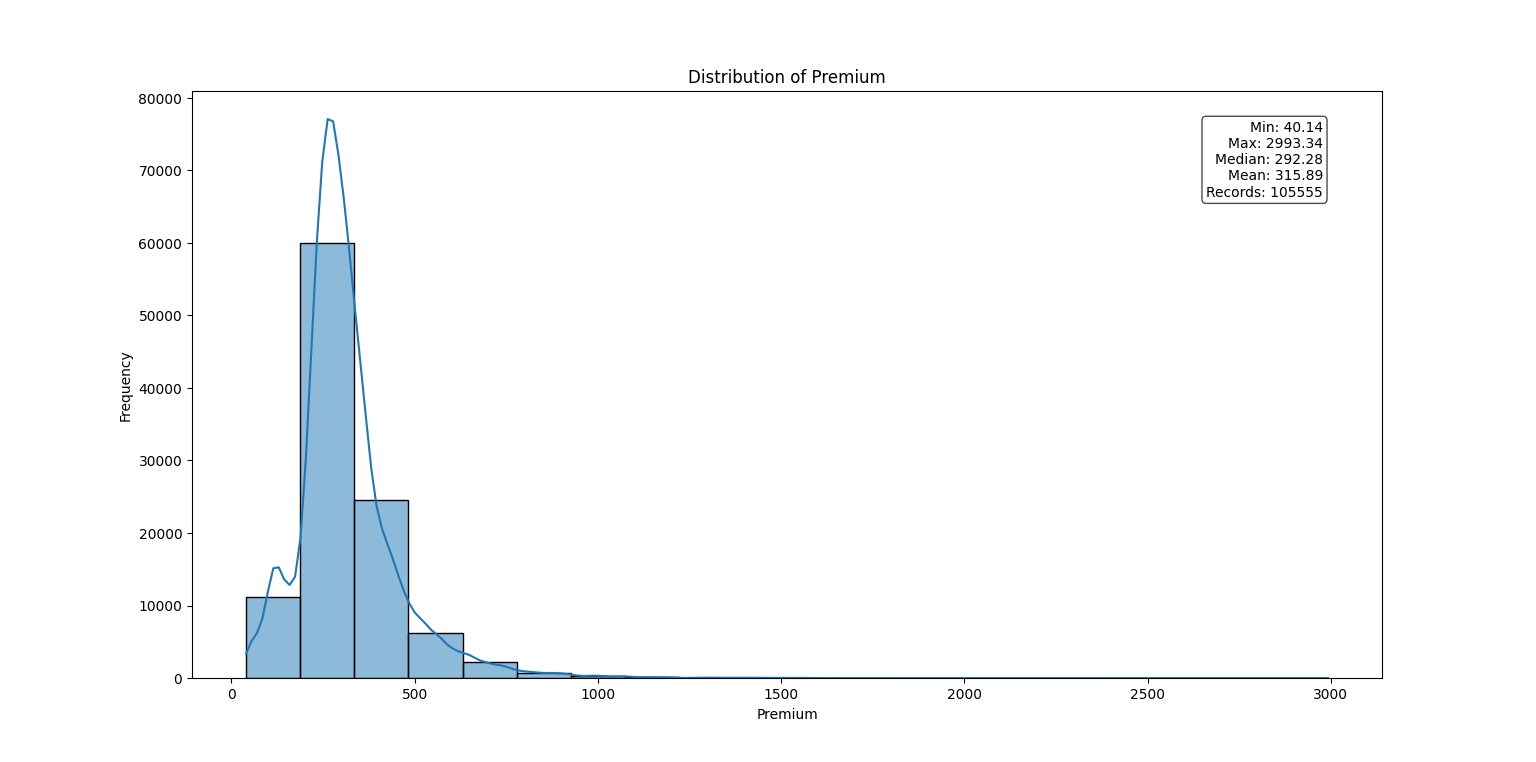
\includegraphics[width=1\textwidth, keepaspectratio]{images/premium.png}

\begin{figure}
    \centering
     \begin{subfigure}{0.45\linewidth}
      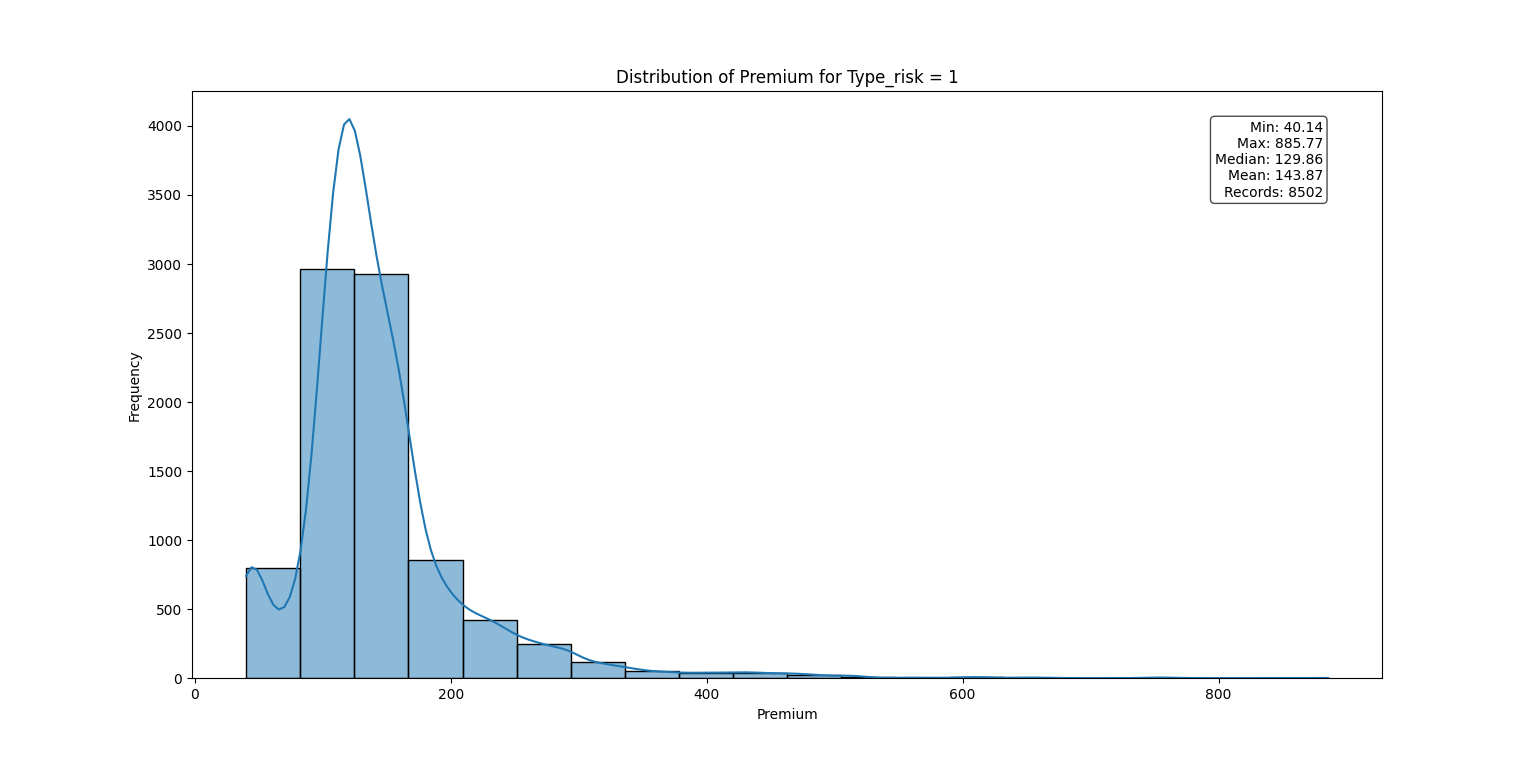
\includegraphics[width=\linewidth]{images/premium_risk1.png}
      \caption{Motorbikes}
      \label{fig:subfig1}
     \end{subfigure}
     \begin{subfigure}{0.45\linewidth}
      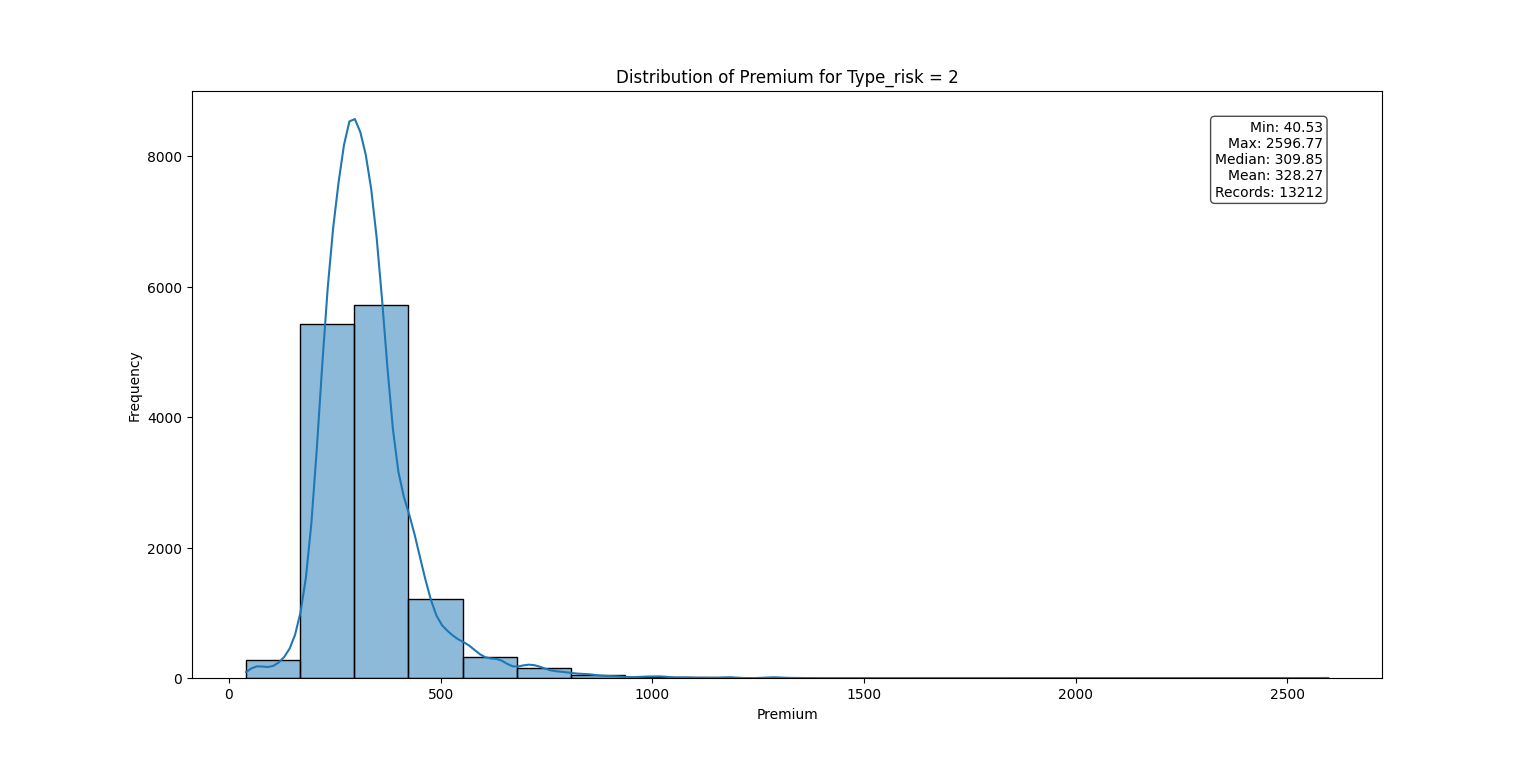
\includegraphics[width=\linewidth]{images/premium_risk2.png}
      \caption{Vans}
      \label{fig:subfig2}
      \end{subfigure}
  \vfill
       \begin{subfigure}{0.45\linewidth}
       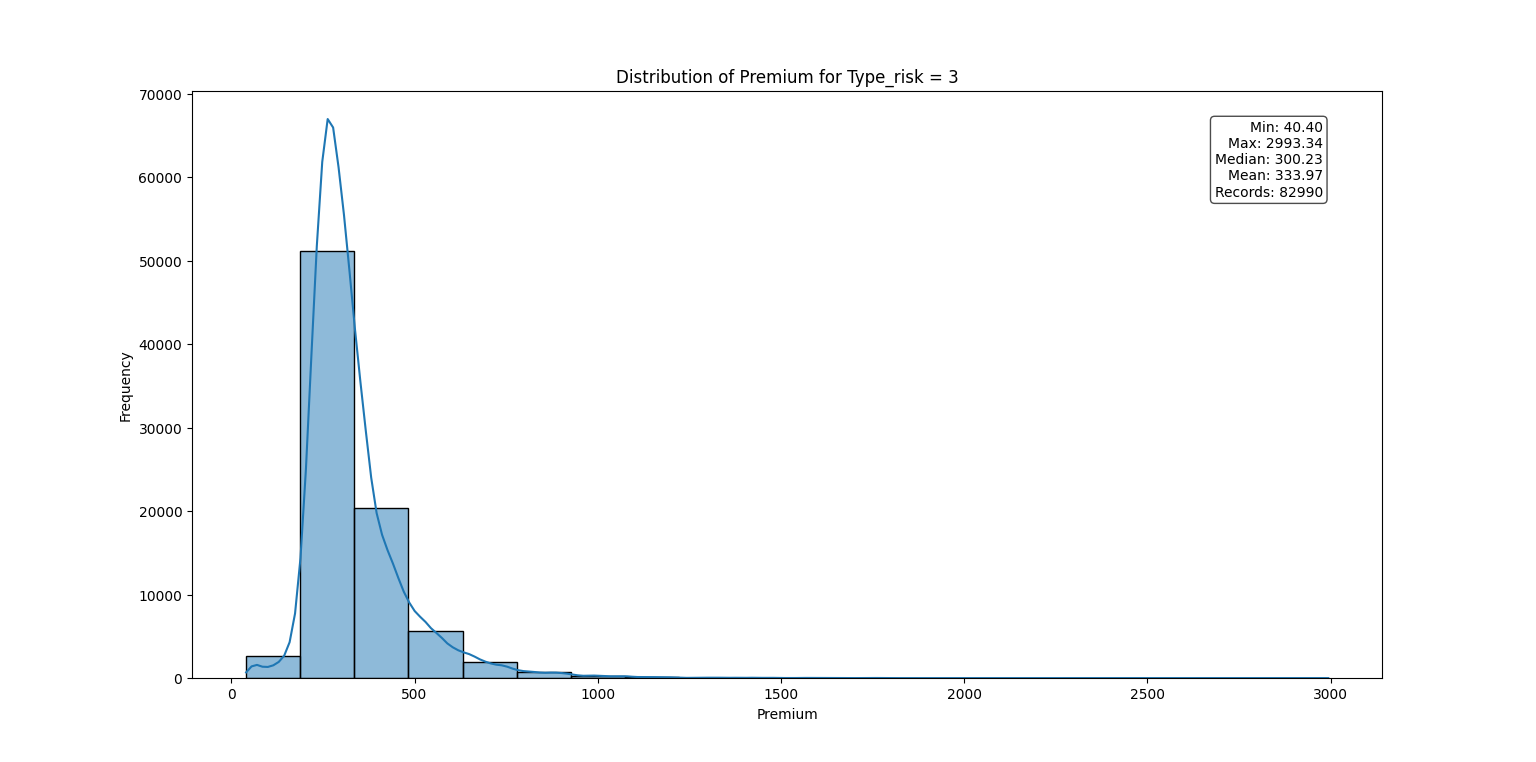
\includegraphics[width=\linewidth]{images/premium_risk3.png}
       \caption{Passenger cars}
       \label{fig:subfig3}
        \end{subfigure}
         \begin{subfigure}{0.45\linewidth}
        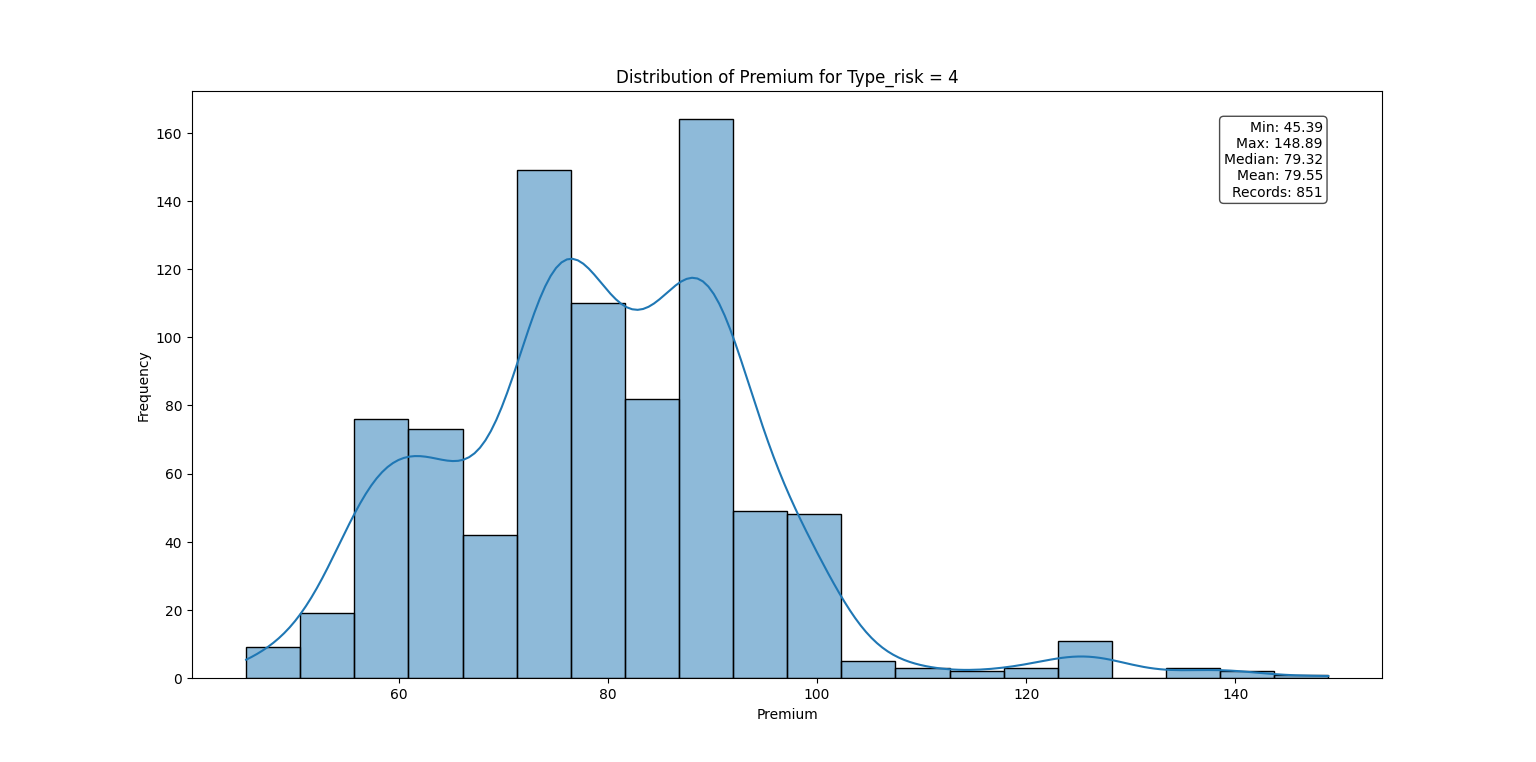
\includegraphics[width=\linewidth]{images/premium_risk4.png}
        \caption{Agricultural Vehicles}
        \label{fig:subfig4}
         \end{subfigure}
  \caption{Comparison of Different Vehicle Types}
  \label{fig:subfigures4}
\end{figure}


\begin{observation}
    Στο πρώτο διάγραμμα παρουσιάζεται η κατανομή των ασφαλίστρων για όλες τις καταχωρίσεις. Τα επόμενα διαγράμματα δείχνουν την κατανομή των ασφαλίστρων για κάθε κατηγορία οχημάτων ξεχωριστά.

    Εύκολα διαπιστώνεται από το πρώτο ολικό διάγραμμα ότι οι ασφαλιστικές τιμές πάνω από 500 είναι ελάχιστες και δεν επηρεάζουν σημαντικά το τελικό αποτέλεσμα. Ωστόσο, όταν κατηγοριοποιήσαμε τα δεδομένα, παρατηρήσαμε ότι η διασπορά των τιμών στα αγροτικά οχήματα ήταν μεγαλύτερη, με αποτέλεσμα η διαφοροποίηση του μοντέλου ανά κατηγορία οχήματος να είναι απαραίτητη.
\end{observation}

\section{User Interface}
Το user interface της εφαρμογής αναπτύχθηκε με χρήση της Python και ειδικότερα του framework Kivy, καθώς και της συλλογής από γραφικά στοιχεία KivyMD. Στην εφαρμογή μας υπάρχουν πέντε διαφορετικές "οθόνες":
\begin{enumerate}
    \item Η οθόνη του login
    \item Η οθόνη συμπλήρωσης στοιχείων του πελάτη που πρόκειται να ασφαλίσει το όχημά του.
    \item Η οθόνη συμπλήρωσης στοιχείων του οχήματος που πρόκειται να ασφαλιστεί.
    \item Η οθόνη συμπλήρωσης στοιχείων παλαιότερων συμβολαίων που είχε ο πελάτης στην εταιρεία.
    \item Η οθόνη παρουσίασης της προτεινόμενης ετήσιας τιμής χρέωσης του πελάτη με βάση τα στοιχεία που συμπληρώθηκαν.
\end{enumerate}

\subsection{Login}
Η οθόνη του login είναι η αρχική οθόνη της εφαρμογής [Εικ. \ref{fig:login}] στην οποία ο χρήστης - υπάλληλος της εταιρείας θα πρέπει να συμπληρώσει τα σωστά στοιχεία συνδεσής του (username και password) και στην συνέχεια να πατήσει το κουμπί "LOG IN". Σε περίπτωση που ένα από τα δύο πεδία μείνει κενό, ο χρήστης θα λάβει το αντίστοιχο μήνυμα λάθους [Εικ. \ref{fig:empty}].
Σε περίπτωση που τα στοιχεία σύνδεσης δεν είναι σωστά, ο χρήστης θα λάβει διαφορετικό μήνυμα λάθους [Εικ. \ref{fig:match}].

Έχει προβλεφθεί και δημιοθργηθεί μόνο ένας λογαριασμός υπαλλήλου. 'Ετσι, για να πάμε στην επόμενη οθόνη θα πρέπει να συμπληρώσουμε στο πεδίο username: \textbf{admin\_1} και στο πεδίο password: \textbf{12345}. Αφού συμπληρώσουμε αυτά τα στοιχεία σωστά και πατήσουμε το κουμπί "LOG IN" μεταφερόμαστε στην δεύτερη οθόνη [Εικ. \ref{fig:driver}].
\begin{figure}
    \begin{center}
        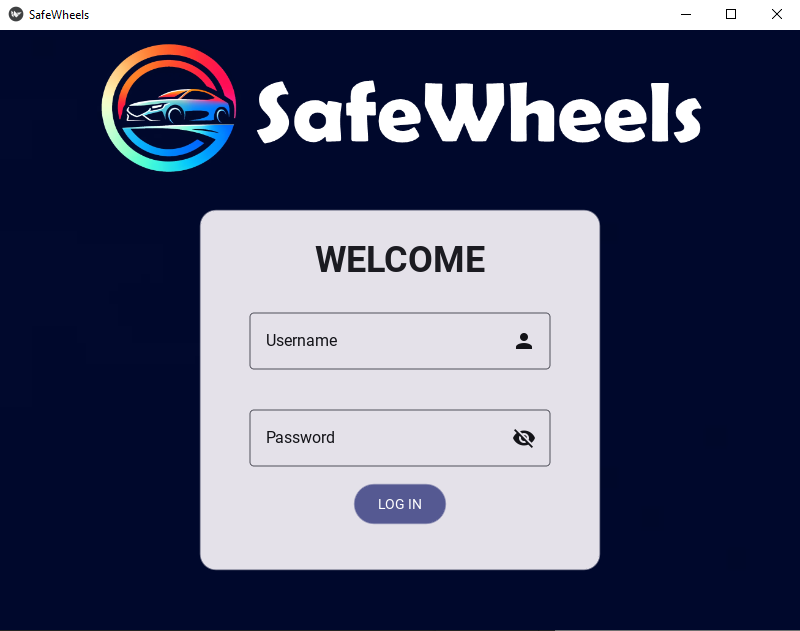
\includegraphics[width=0.6\textwidth]{images/login.png}
    \end{center}
    \caption{Οθόνη login} 
    \label{fig:login}   
\end{figure}

\begin{figure}
    \centering
    \begin{subfigure}{0.45\linewidth}
        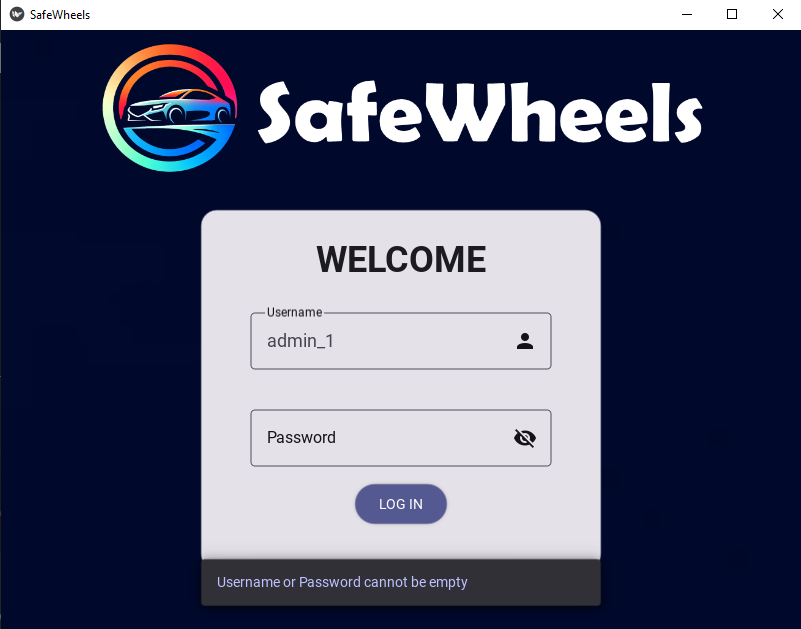
\includegraphics[width=\linewidth]{images/login_empty.png}
        \caption{Κενό πεδίο}
        \label{fig:empty}
    \end{subfigure}
    \begin{subfigure}{0.45\linewidth}
        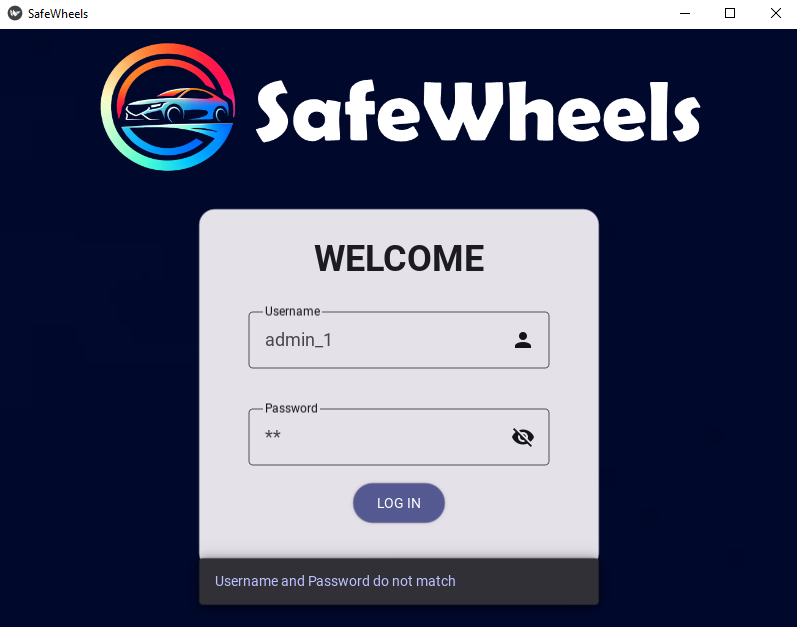
\includegraphics[width=\linewidth]{images/login_dont_match.png}
        \caption{Λάθος στοιχεία}
        \label{fig:match}
    \end{subfigure}
    \caption{Μηνύματα λάθους στο login}
    \label{fig:errors}
\end{figure}
        
\subsection{Στοιχεία πελάτη}
Στην οθόνη συμπλήρωσης στοιχείων του πελάτη [Εικ. \ref{fig:driver}], ο χρήστης-υπάλληλος της εταιρείας θα πρέπει να συμπληρώσει τα στοιχεία του ανθρώπου που ενδιαφέρεται 
να ασφαλίσει το όχημά του. Ειδικότερα, υπάρχουν δύο πεδία επιλογής ημερομηνίας ("Date of Birth", "License Issue Date"), τα οποία όταν επιλεχθούν εμφανίζεται 
ένα ημερολόγιο [Εικ. \ref{fig:date}] προκειμένου να επιλεχθεί η κατάλληλη ημερομηνία. Πατώντας το πεδίο "Area" ο χρήστης βλέπει ένα μενού δύο επιλογών [Εικ. \ref{fig:area}] από τις οποίες θα πρέπει να επιλέξει μία.
Στο πεδίο "Seniority" ο χρήστης θα πρέπει να πληκτρολογήσει έναν αριθμό που προσδιορίζει τα χρόνια που ο συγεκριμένος πελάτης είναι ασφαλισμένος στην εταιρεία. 

Αφού συμπληρωθούν όλα τα πεδία ο χρήστης θα πρέπει να πατήσει το 
κουμπί "NEXT" για να μεταφερθεί στην επόμενη οθόνη [Εικ. \ref{fig:vehicle}]. Σε περίπτωση που επιθυμεί να πάει στην οθόνη του login [Εικ. \ref{fig:login}] θα πρέπει να πατήσει το κουμπί "GO BACK".

\begin{figure}
    \begin{center}
        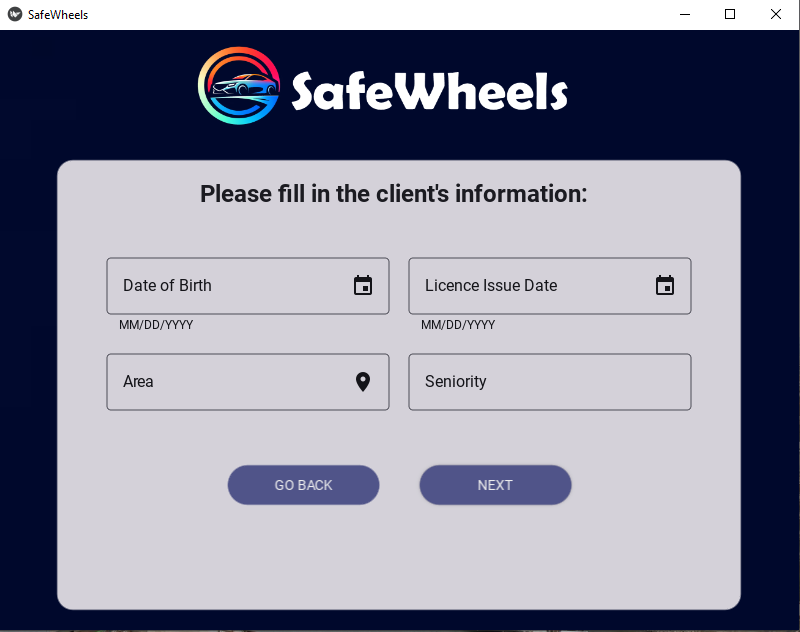
\includegraphics[width=0.6\textwidth]{images/driver.png}
    \end{center}
    \caption{Οθόνη συμπλήρωσης στοιχείων πελάτη}  
    \label{fig:driver}  
\end{figure}

\begin{figure}
    \centering
    \begin{subfigure}{0.45\linewidth}
        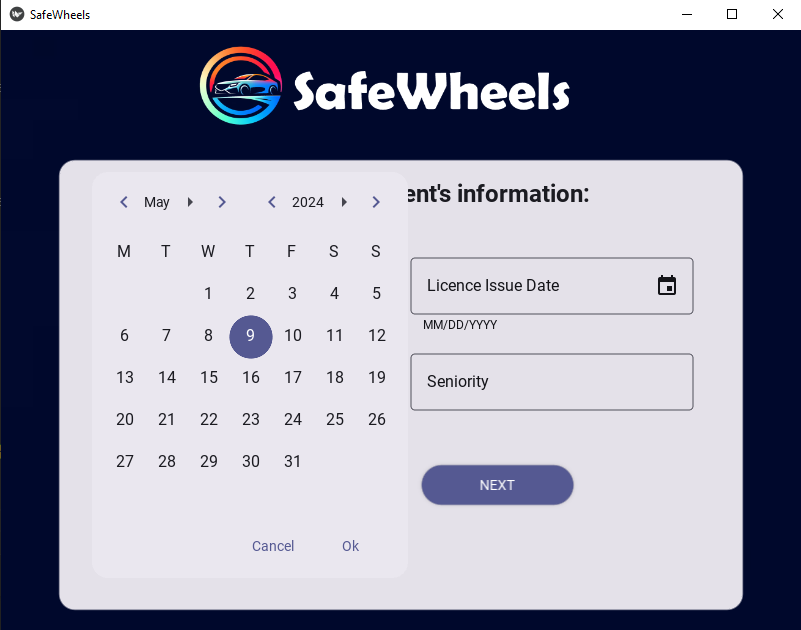
\includegraphics[width=\linewidth]{images/driver_datepicker.png}
        \caption{Ημερολόγιο}
        \label{fig:date}
    \end{subfigure}
    \begin{subfigure}{0.45\linewidth}
        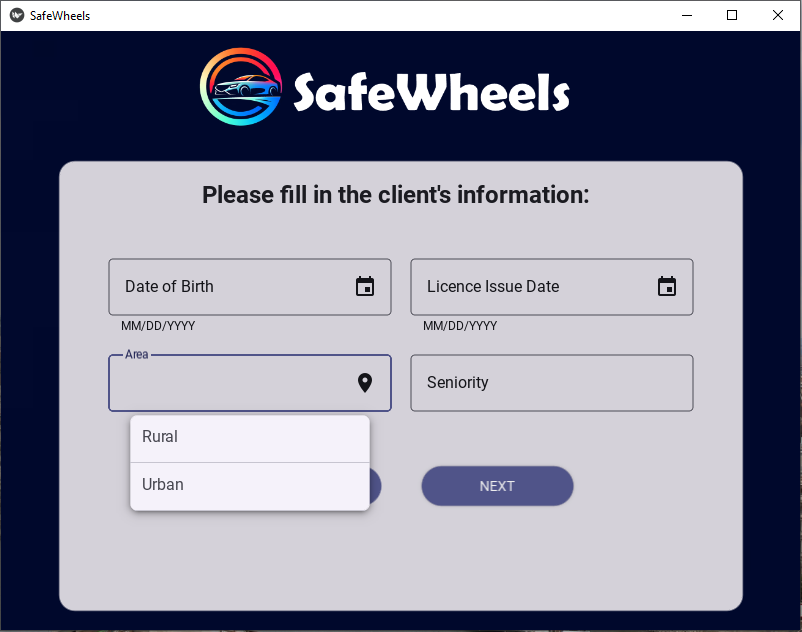
\includegraphics[width=\linewidth]{images/driver_area.png}
        \caption{Μενού επιλογών}
        \label{fig:area}
    \end{subfigure}
    \caption{Παραδείγματα εισόδου}
    \label{fig:driver_examples}
\end{figure}


\subsection{Στοιχεία οχήματος}
Σε αυτήν την οθόνη [Εικ. \ref{fig:vehicle}], ο χρήστης-υπάλληλος της εταιρείας θα πρέπει να συμπληρώσει τα στοιχεία του οχήματος το οποίο επιθυμεί να ασφαλίσει ο πελάτης. Ειδικότερα, για τα πεδία 
"Type of vehicle", "Type of fuel", "Second driver" ο χρήστης θα πρέπει να πατήσει καθένα από αυτά τα πεδία και να επιλέξει μία από τις επιλογές που εμφανίζονται στο κάθε μενού επιλογών (ενδεικτικά [Εικ. \ref{fig:type}]). 
Στα υπόλοιπα πεδία ο χρήστης θα πρέπει να πληκτρολογήσει έναν αριθμό σύμφωνα με τις υποδείξεις του κάθε πεδίου (ενδεικτικά [Εικ. \ref{fig:reg}]).

Για να μεταβεί στην επόμενη οθόνη [Εικ. \ref{fig:contract}] θα πρέπει να πατήσει το κουμπί "NEXT" ενώ για να πάει στην προηγούμενη οθόνη [Εικ. \ref{fig:driver}] συμπλήρωσης των στοιχείων του πελάτη θα πρέπει να πατήσει το κουμπί "GO BACK".

\begin{figure}
    \begin{center}
        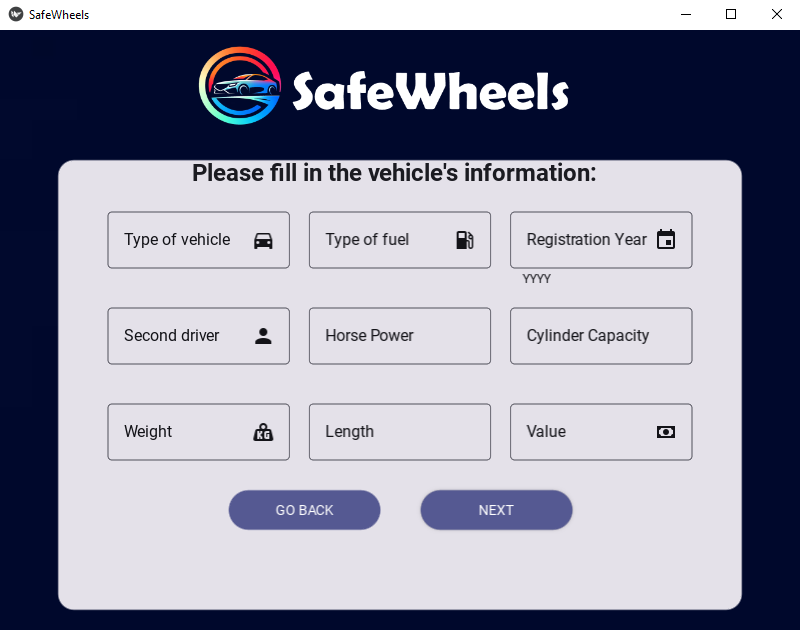
\includegraphics[width=0.6\textwidth]{images/vehicle.png}
    \end{center}
    \caption{Οθόνη συμπλήρωσης στοιχείων οχήματος προς ασφάλιση}  
    \label{fig:vehicle}  
\end{figure}

\begin{figure}
    \centering
    \begin{subfigure}{0.45\linewidth}
        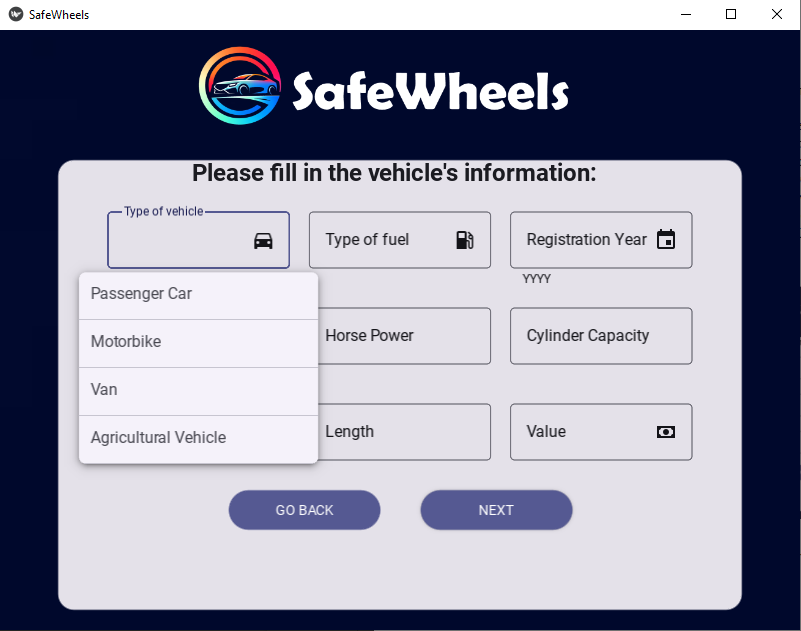
\includegraphics[width=\linewidth]{images/vehicle_type.png}
        \caption{Παράδειγμα μενού επιλογών}
        \label{fig:type}
    \end{subfigure}
    \begin{subfigure}{0.45\linewidth}
        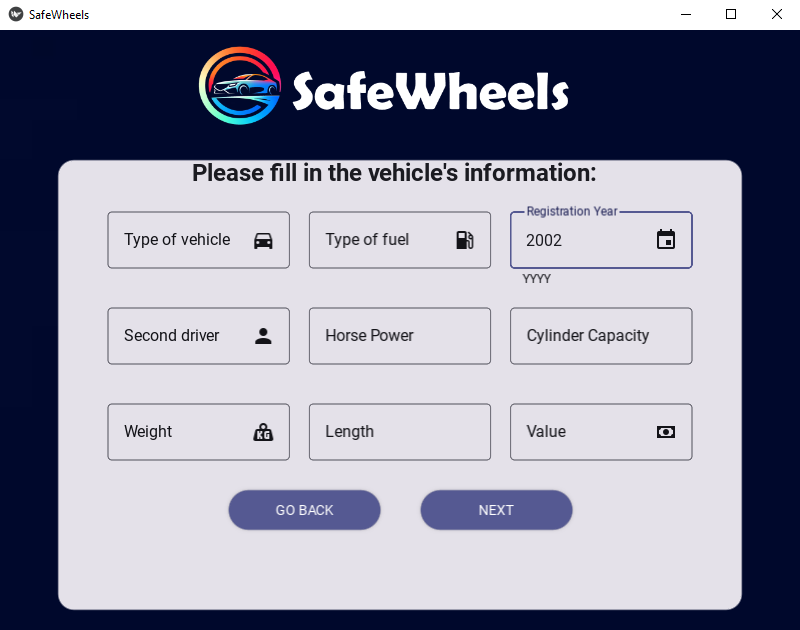
\includegraphics[width=\linewidth]{images/vehicle_reg_year.png}
        \caption{Παράδειγμα συμπλήρωσης πεδίου}
        \label{fig:reg}
    \end{subfigure}
    \caption{Παραδείγματα εισόδου}
    \label{fig:vehicle_examples}
\end{figure}

\newpage
\subsection{Στοιχεία συμβολαίου}
Στην οθόνη συμπληρωσης στοιχείων συμβολαίου [Εικ. \ref{fig:contract}] ο χρήστης-υπάλληλος της εταιρείας θα πρέπει να συμπληρώσει στοιχεία που αφορούν παλαιότερα συμβόλαια που είχε ο πελάτης στην εταιρεία.
Υπάρχουν τρία πεδία επιλογής ημερομηνίας ("Start Contract", "Last renewal", "Next renewal"), τα οποία όταν επιλεχθούν εμφανίζεται ημερολόγιο (ενδεικτικά [Εικ. \ref{fig:con_date}]). Τα πεδία "Distribution Channel" και "Payment" είναι πεδία που
κατά την επιλογή τους εμφανίζεται μενού επιλογών (ενδεικτικά [Εικ. \ref{fig:pay}]), ενώ τα υπόλοιπα πρέπει να συμπληρωθούν με πληκτρολόγηση σύμφωνα με τις υποδείξεις των πεδίων.

Για την μετάβαση στην προηγούμενη οθόνη [Εικ. \ref{fig:vehicle}] ο χρήστης θα πρέπει να πατήσει το κουμπί "GO BACK". Διαφορετικά, βρισκόμαστε στο σημείο που έχουν συμπληρωθεί όλα τα στοιχεία και ο χρήστης θα πρέπει να πατήσει το 
κουμπί "CALCULATE" προκειμένου να μεταβεί στην τελευταία οθόνη [Εικ. \ref{fig:premium}].

\begin{figure}
    \begin{center}
        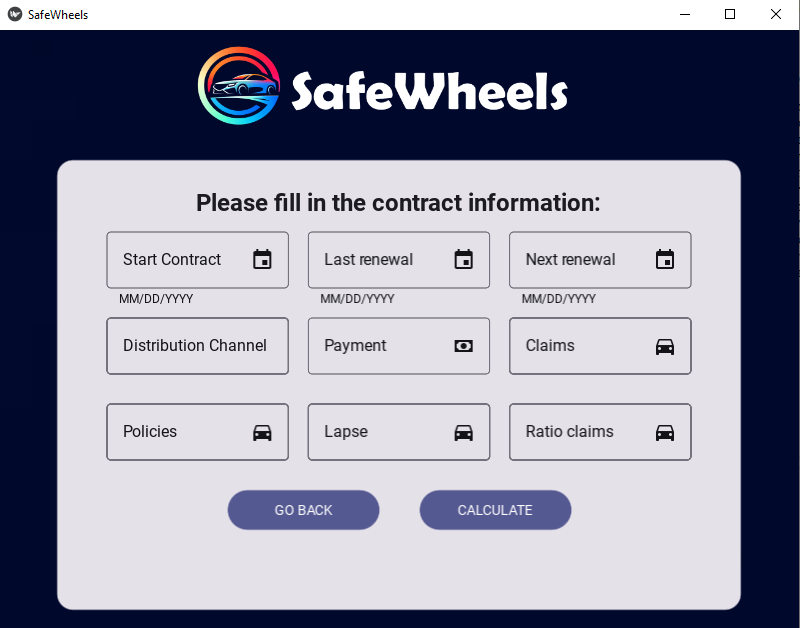
\includegraphics[width=0.6\textwidth]{images/contract.png}
    \end{center}
    \caption{Οθόνη συμπλήρωσης στοιχείων οχήματος προς ασφάλιση}  
    \label{fig:contract}  
\end{figure}

\begin{figure}
    \centering
    \begin{subfigure}{0.45\linewidth}
        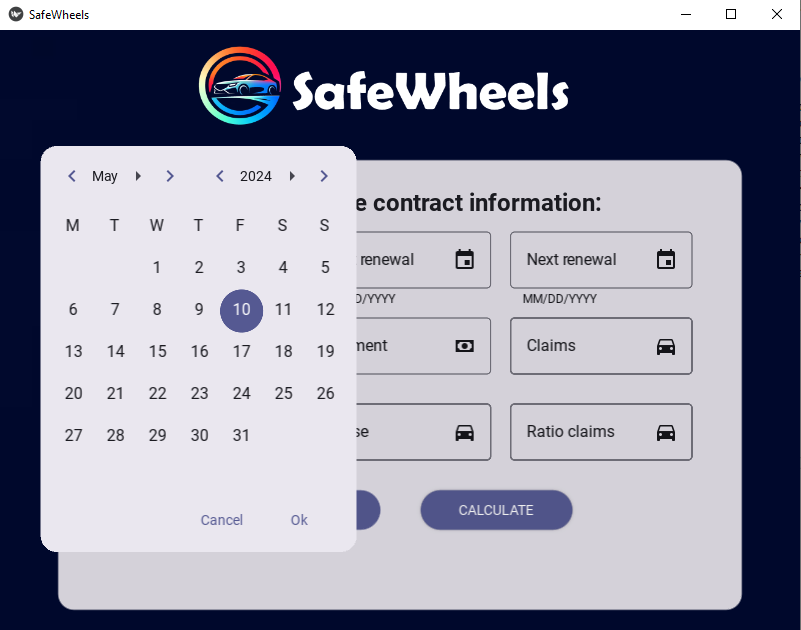
\includegraphics[width=\linewidth]{images/contract_date.png}
        \caption{Παράδειγμα ημερολογίου}
        \label{fig:con_date}
    \end{subfigure}
    \begin{subfigure}{0.45\linewidth}
        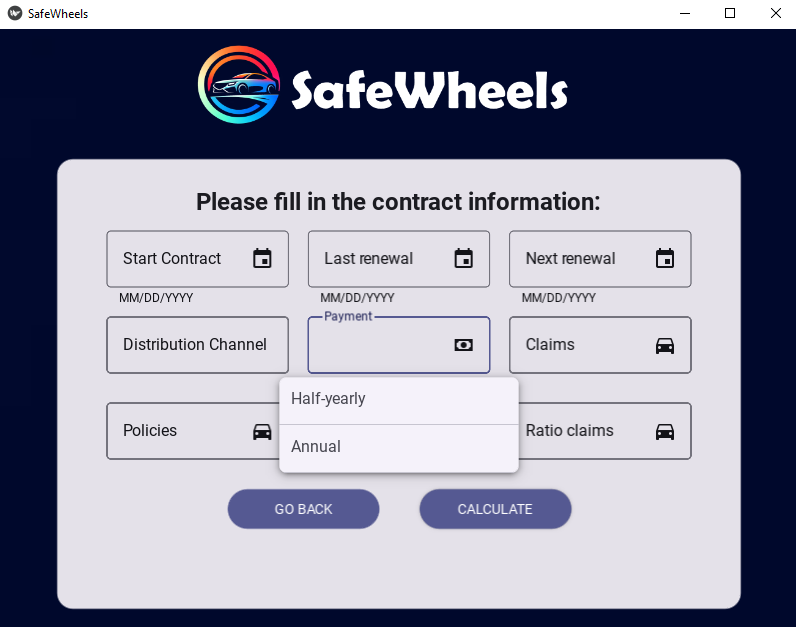
\includegraphics[width=\linewidth]{images/contract_pay.png}
        \caption{Παράδειγμα μενού επιλογών}
        \label{fig:pay}
    \end{subfigure}
    \caption{Παραδείγματα εισόδου}
    \label{fig:contract_examples}
\end{figure}

\newpage
\subsection {Οθόνη προτινόμενης χρέωσης}
Σε αυτήν την οθόνη [Εικ. \ref{fig:premium}], ο χρήστης-υπάλληλος της εταιρείας βλέπει την προτεινόμενη τιμή ασφάλισης του οχήματος που πρόκειται να ασφαλίσει ο πελάτης.
Πατώντας το κουμπί "GO BACK" μπορεί να μεταβεί στην προήγουμενη οθόνη [Εικ. \ref{fig:contract}], ενώ πατώντας το κουμπί "LOGOUT" μεταβαίνει στην αρχική οθόνη της εφαρμογής [Εικ. \ref{fig:login}].

Αξίζει να σημειωθεί πως ο χρήστης μπορεί να πηγαίνει προς τα πίσω και να αλλάζει στοιχεία ανά πάσα στιγμή. Κάθε φορά που πατά το κουμπί "CALCULATE" της προτελευταίας οθόνης [Εικ. \ref{fig:contract}], 
όλα τα ανανεωμένα στοιχεία δίνονται στο μοντέλο προκειμένου να βγει η προτεινόμενη τιμή χρέωσης.

\begin{figure}
    \begin{center}
        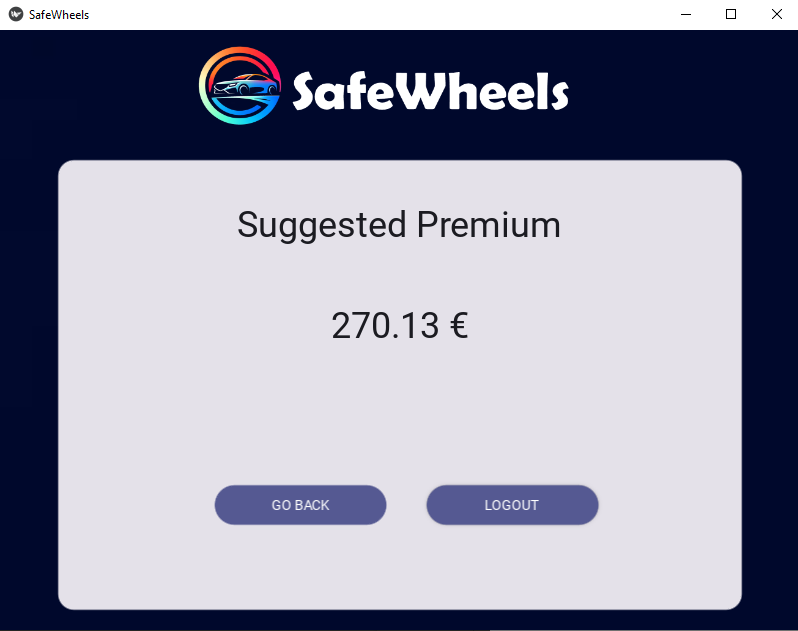
\includegraphics[width=0.6\textwidth]{images/suggested_premium.png}
    \end{center}
    \caption{Οθόνη παρουσίασης προτεινόμενης τιμής χρέωσης}  
    \label{fig:premium}  
\end{figure}

\subsection{Γενικές παρατηρήσεις για το ui}
//κενά πεδία


\section{Oπτικοποίηση και αξιολόγηση αποτελεσμάτων}

Για την αξιολόγηση των μοντέλων χρησιμοποιήσαμε το mean squared error, το absolute error και το ποσοστό των προβλέψεων που 
ήταν εντός της πραγματικής τιμής. Τα αποτελέσματα για κάθε μοντέλο όταν έχει εκπαιδευθεί στο σύνολο των δεδομένων:

\begin{table}[h]
    \centering
    \begin{tabular}{|c|c|c|c|} % 4 columns
        \hline
         &Mean squared error & Absolute error & Percentage within 10\% \\ % 4 rows
        \hline
        XGBoost & 10370.87 & 66.19 & 34.87 \\
        Random Forest & 10852.02 & 67.38 & 33.36 \\
        Neural network & 11689.55 & 70.16 & 20.00 \\
        \hline
    \end{tabular}
    \caption{Αξιολόγηση των μοντέλων}
    \label{tab:3x3table}
\end{table}

\begin{figure}
    \begin{center}
        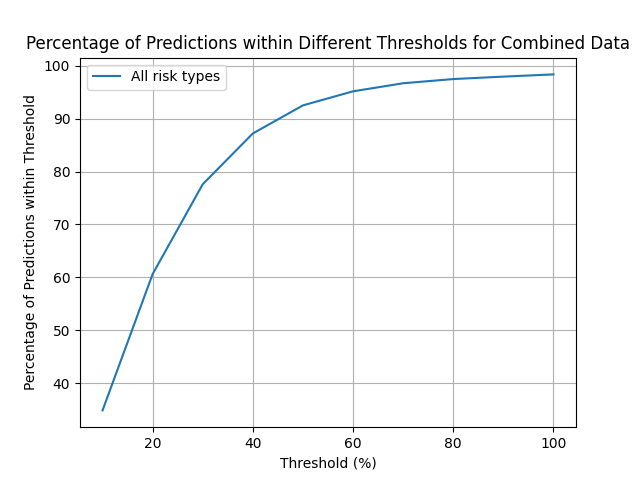
\includegraphics[width=0.6\textwidth]{images/combined_trained_all_thresholds_xgb.png}
    \end{center}
    \caption{Μοντέλο XGBoost που εκπαιδεύτηκε στο σύνολο των δεδομένων}  
    \label{fig:XGBoost_result}  
\end{figure}

\begin{figure}
    \begin{center}
        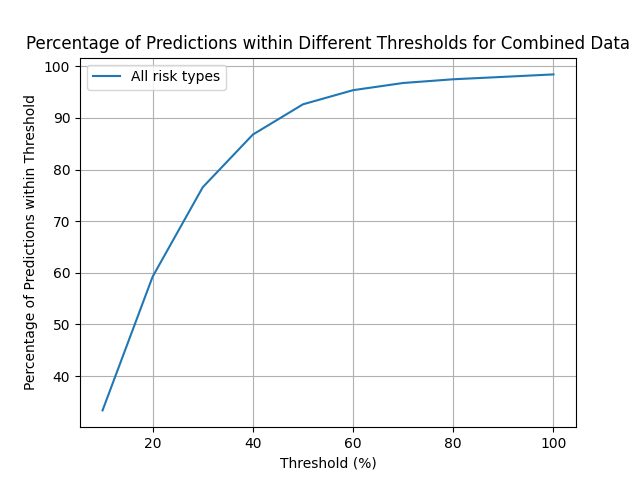
\includegraphics[width=0.6\textwidth]{images/combined_trained_all_thresholds_random_forest.png}
    \end{center}
    \caption{Μοντέλο Random Forest που εκπαιδεύτηκε στο σύνολο των δεδομένων}  
    \label{fig:random_forest_result}  
\end{figure}

\begin{figure}
    \begin{center}
        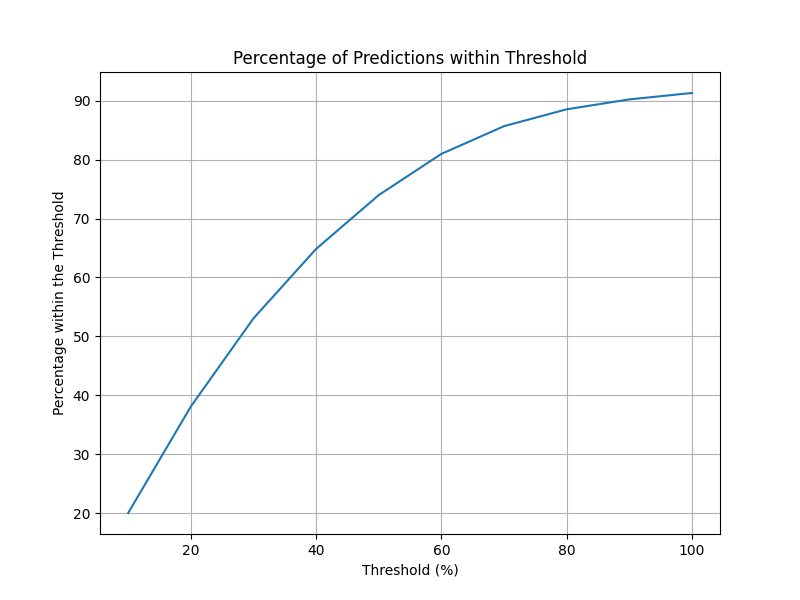
\includegraphics[width=0.6\textwidth]{images/neural_network_all_thresholds.png}
    \end{center}
    \caption{Μοντέλο Νευρωνικού δικτύου που εκπαιδεύτηκε στο σύνολο των δεδομένων}  
    \label{fig:neural_result}  
\end{figure}


Από αυτής την αξιολόγηση φαίνετε ότι το πιο ακριβές μοντέλο
είναι το XGBoost.

Παρατηρήσαμε ότι υπάρχουν στα δεδομένα μας 4 διαφορετικές κατηγορίες οχήματων και
για τα μοντέλα του Random Forest και XGBoost που έχουν εκπαιδευθεί στον σύνολο τον δεδομένων
κάναμε ξεχωριστή αξιολόγηση ανα κατηγορία.
\begin{table}[h]
    \centering
    \begin{tabular}{|c|c|c|c|} % 4 columns
        \hline
         &Mean squared error & Absolute error & Percentage within 10\% \\ % 4 rows
        \hline
        Μοτοσυκλέτα & 2358.08 & 30.92 & 35.25 \\
        Βανάκι & 8266.77 & 61.80 & 37.50 \\
        Επιβατικό όχημα & 11574.03 & 70.76 & 34.50 \\
        Αγροτικό όχημα & 2348.79 & 27.96 & 26.92 \\
        \hline
    \end{tabular}
    \caption{Αξιολόγηση XGBoost ανα κατηγορία}
    \label{tab:XGBoost_cat_together}
\end{table}

\begin{table}[h]
    \centering
    \begin{tabular}{|c|c|c|c|} % 4 columns
        \hline
         &Mean squared error & Absolute error & Percentage within 10\% \\ % 4 rows
        \hline
        Μοτοσυκλέτα & 2229.48 & 29.05 & 36.54 \\
        Βανάκι & 8586.59 & 62.96 & 36.57 \\
        Επιβατικό όχημα & 12159.72 & 72.34 & 32.58 \\
        Αγροτικό όχημα & 829.67 & 20.90 & 29.48 \\
        \hline
    \end{tabular}
    \caption{Αξιολόγηση Random Forest ανα κατηγορία}
    \label{tab:RandomForest_cat_together}
\end{table}


\begin{figure}
    \begin{center}
        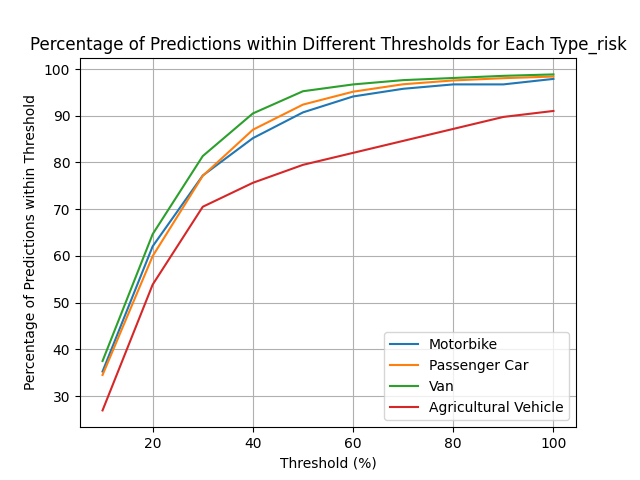
\includegraphics[width=0.6\textwidth]{images/combined_trained_individual_thresholds_xgb.png}
    \end{center}
    \caption{Μοντέλο XGBoost που εκπαιδεύτηκε στο σύνολο των δεδομένων ξεχωριστή αξιολόγηση}  
    \label{fig:XGBoost_result_all_individual}  
\end{figure}

\begin{figure}
    \begin{center}
        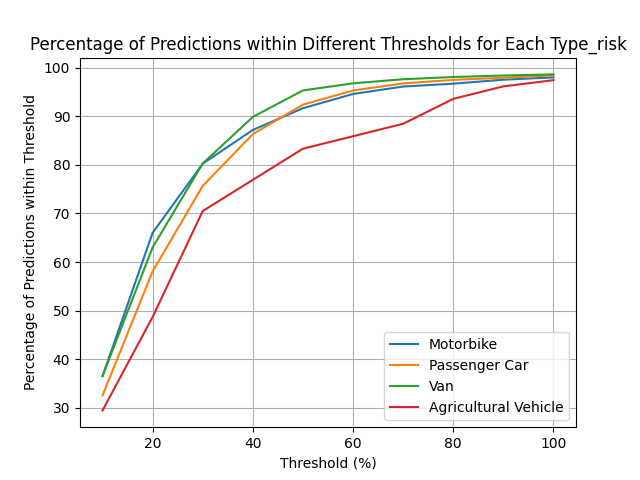
\includegraphics[width=0.6\textwidth]{images/combined_trained_individual_thresholds_random_forest.png}
    \end{center}
    \caption{Μοντέλο Random Forest που εκπαιδεύτηκε στο σύνολο των δεδομένων ξεχωριστή αξιολόγηση}  
    \label{fig:random_forest_result_all_individual}  
\end{figure}


Όπως εξηγήσαμε και στην εκπαίδευση των μοντέλων αποφασήσαμε να μοιράσουμε τα 
δεδομένα στις τέσσερις κατηγορίες και να εκπεδαίυσουμε ένα μοντέλο για την καθεμία
και όντως η ακρίβεια των μοντέλων αυξήθηκε 

\begin{figure}
    \begin{center}
        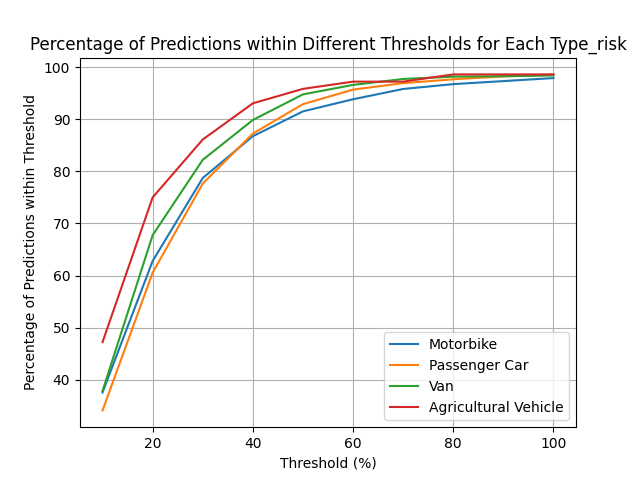
\includegraphics[width=0.6\textwidth]{images/individual_thresholds_xgb.png}
    \end{center}
    \caption{Μοντέλο XGBoost που εκπαιδεύτηκε ξεχωριστά για κάθε κατηγορία}  
    \label{fig:XGBoost_result_cat}  
\end{figure}

\begin{figure}
    \begin{center}
        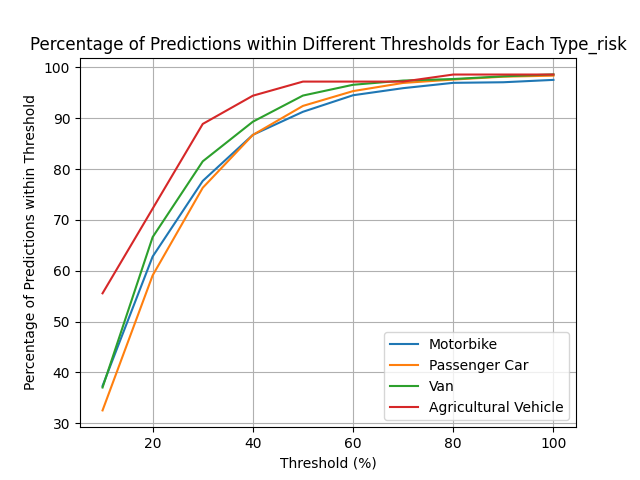
\includegraphics[width=0.6\textwidth]{images/individual_thresholds_random_forest.png}
    \end{center}
    \caption{Μοντέλο Random Forest που εκπαιδεύτηκε ξεχωριστά για κάθε κατηγορία}  
    \label{fig:random_forest_result_cat}  
\end{figure}

\begin{figure}
    \begin{center}
        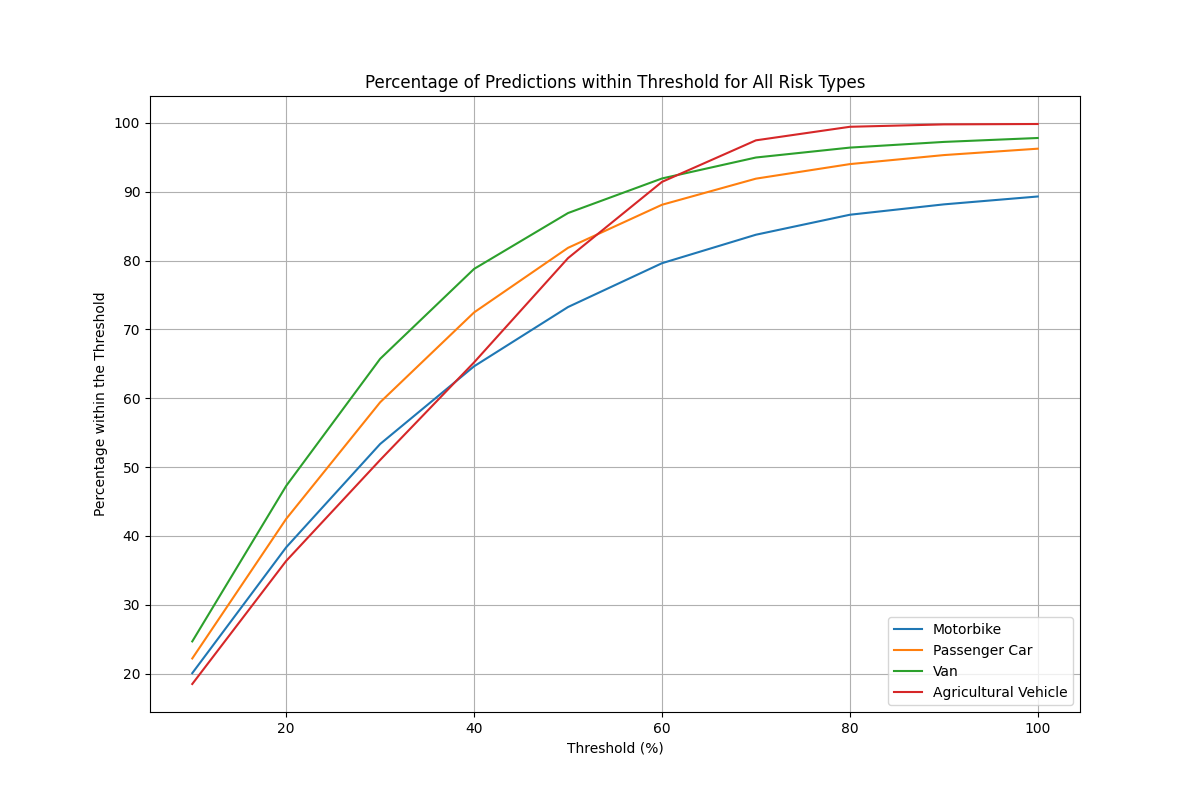
\includegraphics[width=0.6\textwidth]{images/individual_thresholds_neural.png}
    \end{center}
    \caption{Μοντέλο Νευρωνικού δικτύου που εκπαιδεύτηκε ξεχωριστά για κάθε κατηγορία}  
    \label{fig:neural_result_cat}  
\end{figure}

\begin{table}[h]
    \centering
    \begin{tabular}{|c|c|c|c|} % 4 columns
        \hline
         &Mean squared error & Absolute error & Percentage within 10\% \\ % 4 rows
        \hline
        Μοτοσυκλέτα & 2228.74 & 29.77 & 38.13 \\
        Βανάκι & 7846.43 & 60.34 & 38.07 \\
        Επιβατικό όχημα & 10693.59 & 69.07 & 33.66 \\
        Αγροτικό όχημα & 311.89 & 12.15 & 51.38 \\
        \hline
    \end{tabular}
    \caption{Αξιολόγηση XGBoost ανα κατηγορία}
    \label{tab:XGBoost_cat_individual}
\end{table}

\begin{table}[h]
    \centering
    \begin{tabular}{|c|c|c|c|} % 4 columns
        \hline
         &Mean squared error & Absolute error & Percentage within 10\% \\ % 4 rows
        \hline
        Μοτοσυκλέτα & 2265.09 & 29.42 & 37.32 \\
        Βανάκι & 8184.89 & 61.39 & 37.01 \\
        Επιβατικό όχημα & 10923.63 & 70.22 & 32.51 \\
        Αγροτικό όχημα & 267.00 & 11.47 & 55.55 \\
        \hline
    \end{tabular}
    \caption{Αξιολόγηση Random Forest ανα κατηγορία}
    \label{tab:RandomForest_cat_individual}
\end{table}

\begin{table}[h]
    \centering
    \begin{tabular}{|c|c|c|c|} % 4 columns
        \hline
         &Mean squared error & Absolute error & Percentage within 10\% \\ % 4 rows
        \hline
        Μοτοσυκλέτα & 3391.05 & 36.22 & 20.46 \\
        Βανάκι & 8966.14 & 62.96 & 23.95 \\
        Επιβατικό όχημα & 11465.31 & 71.66 & 22.41 \\
        Αγροτικό όχημα & 1325.41 & 29.64 & 12.73 \\
        \hline
    \end{tabular}
    \caption{Αξιολόγηση Νευρωνικού δικτύου ανα κατηγορία}
    \label{tab:neural_network_cat_individual}
\end{table}

Παρατηρούμε ότι το αποτέλεσμα βελτιώθηκε για το το XGBoost και το Random Forest ενώ χειροτέρεψε για το Νευρωνικό δίκτυο.
Το καλύτερο μοντέλο είναι το XGBoost που εκπαιδεύτηκε ξεχωριστά για κάθε κατηγορία
για αυτό επιλέξαμε να το χρησιμοποιήσουμε και για την εφαρμογή μας.

Επίσης για το XGBoost και το Random Forest κάναμε ανάλυση της σημαντικότητας 
των μεταβλητών και για όταν τα μοντέλα εκπαιδεύτηκαν σε όλα τα δεδομένα και όταν είναι χωρισμένα σε κατηγορίες.

\begin{figure}
    \begin{center}
        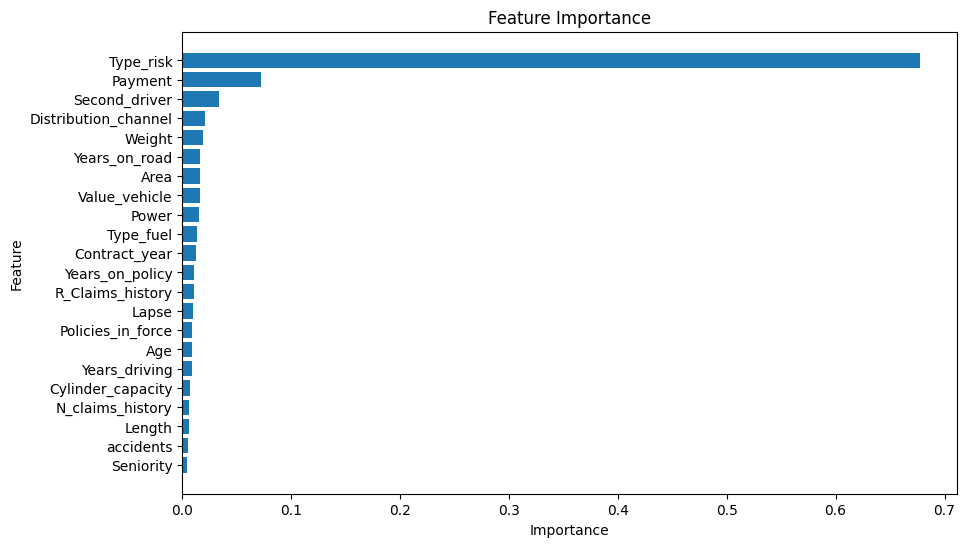
\includegraphics[width=0.6\textwidth]{images/feature_importance_combined_xgb.png}
    \end{center}
    \caption{Μοντέλο XGBoost που εκπαιδεύτηκε σε όλα τα δεδομένα}  
    \label{fig:XGBoost_all_feature_importance}  
\end{figure}

\begin{figure}
    \begin{center}
        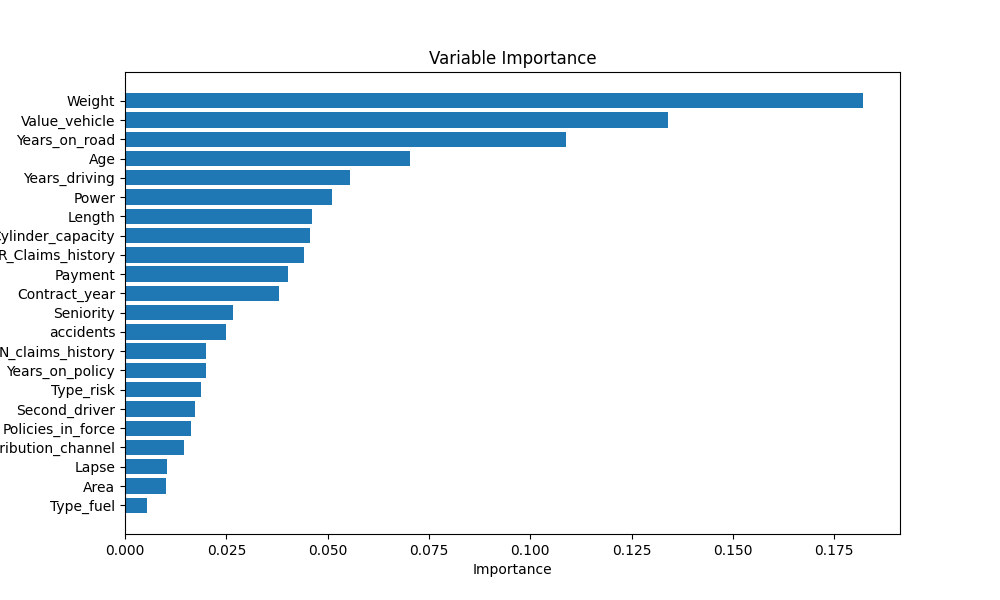
\includegraphics[width=0.6\textwidth]{images/feature_importance_combined_random_forest.png}
    \end{center}
    \caption{Μοντέλο Random Forest που εκπαιδεύτηκε σε όλα τα δεδομένα}  
    \label{fig:random_forest_all_feature_importance}  
\end{figure}

\begin{figure}
    \centering
     \begin{subfigure}{0.45\linewidth}
      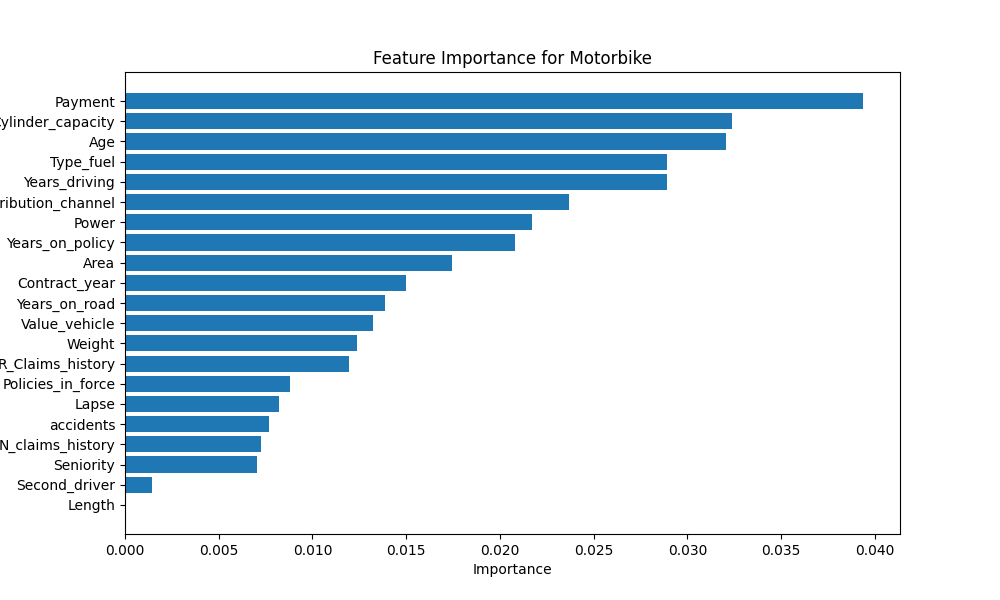
\includegraphics[width=\linewidth]{images/Motorbike_feature_importance_xgb.png}
      \caption{Motorbikes}
      \label{fig:subxgb1}
     \end{subfigure}
     \begin{subfigure}{0.45\linewidth}
      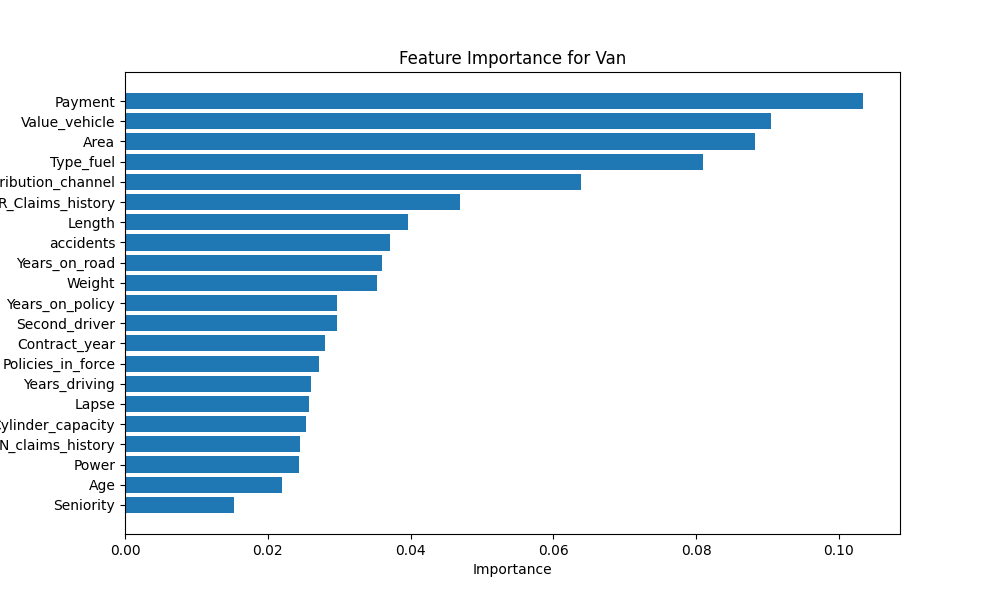
\includegraphics[width=\linewidth]{images/Van_feature_importance_xgb.png}
      \caption{Vans}
      \label{fig:subxgb2}
      \end{subfigure}
  \vfill
       \begin{subfigure}{0.45\linewidth}
       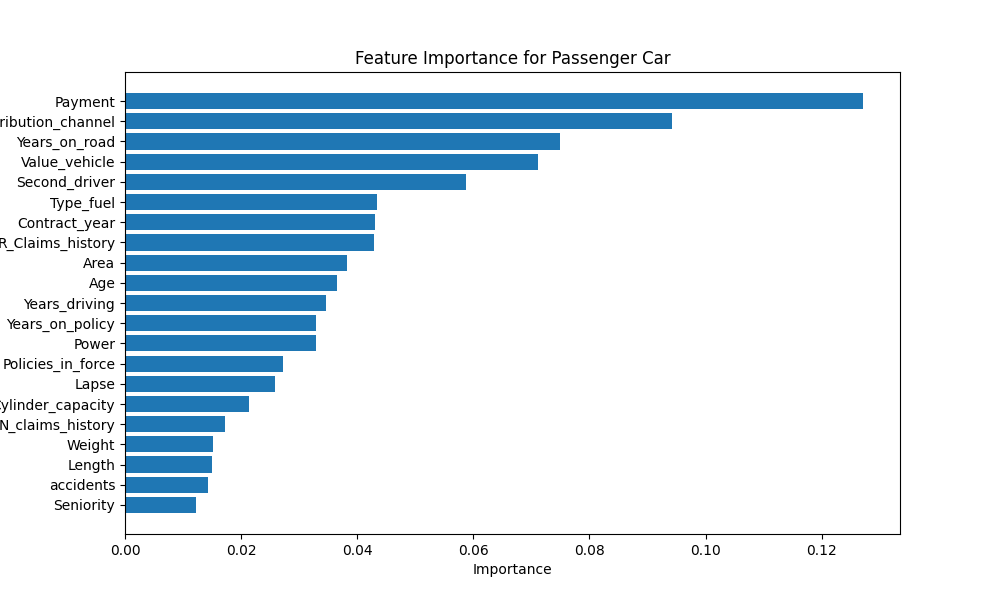
\includegraphics[width=\linewidth]{images/Passenger Car_feature_importance_xgb.png}
       \caption{Passenger cars}
       \label{fig:subxgb3}
        \end{subfigure}
         \begin{subfigure}{0.45\linewidth}
        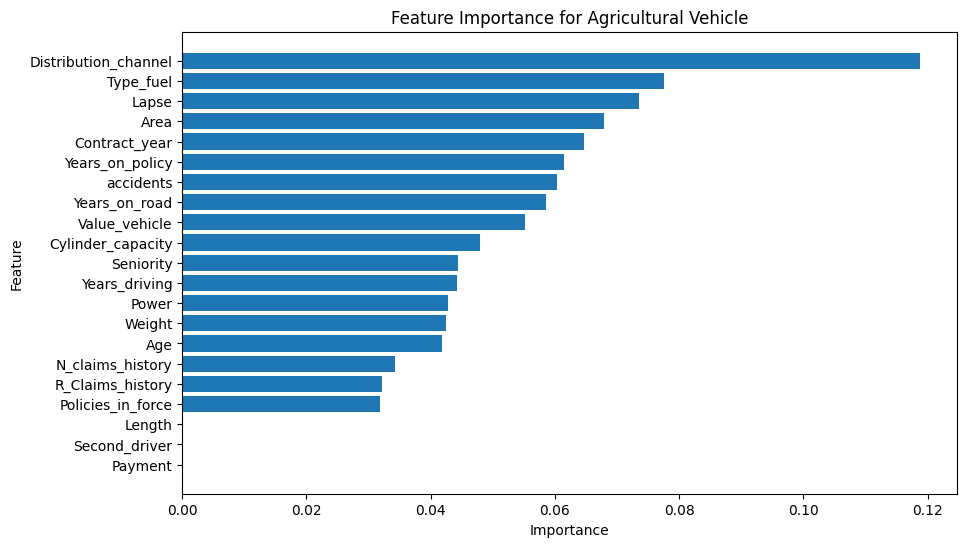
\includegraphics[width=\linewidth]{images/Agricultural Vehicle_feature_importance_xgb.png}
        \caption{Agricultural Vehicles}
        \label{fig:subxgb4}
         \end{subfigure}
  \caption{Μοντέλο XGBoost που εκπαιδεύτηκε ξεχωριστά ανα κατηγορία}
  \label{fig:xgb_split_importance}
\end{figure}

\begin{figure}
    \centering
     \begin{subfigure}{0.45\linewidth}
      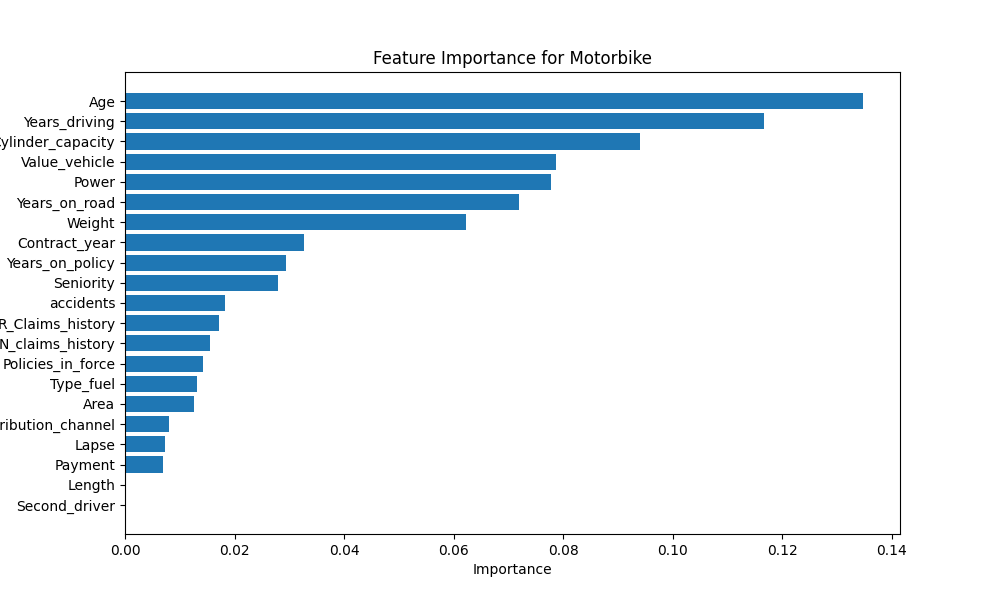
\includegraphics[width=\linewidth]{images/Motorbike_feature_importance_random_forest.png}
      \caption{Motorbikes}
      \label{fig:subrandom1}
     \end{subfigure}
     \begin{subfigure}{0.45\linewidth}
      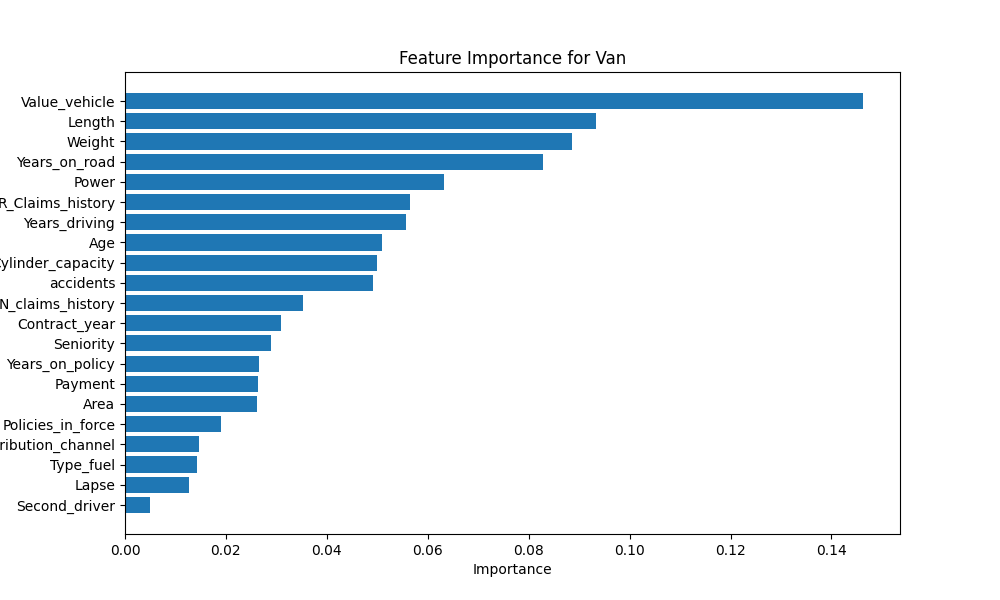
\includegraphics[width=\linewidth]{images/Van_feature_importance_random_forest.png}
      \caption{Vans}
      \label{fig:subrandom2}
      \end{subfigure}
  \vfill
       \begin{subfigure}{0.45\linewidth}
       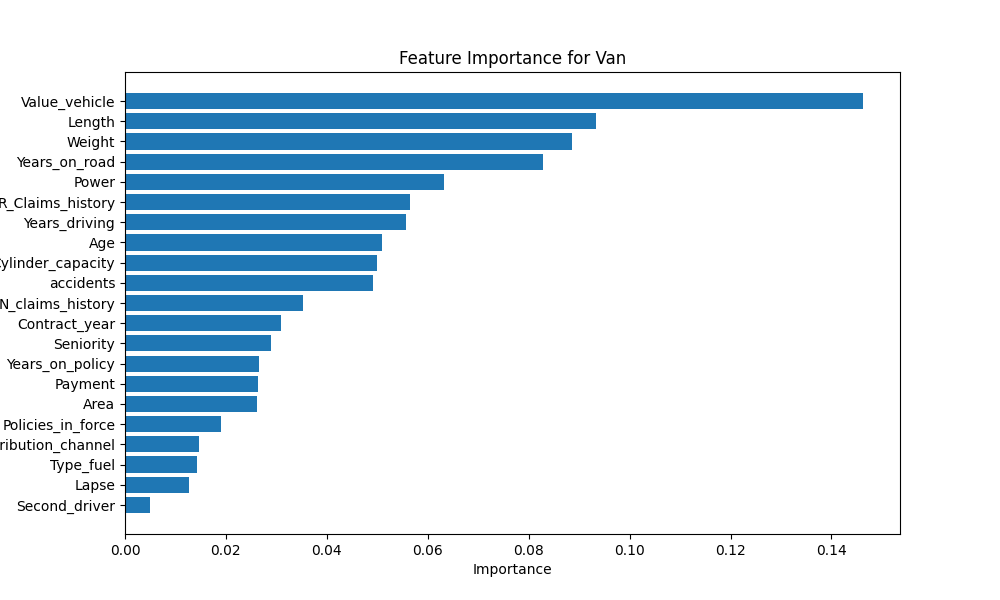
\includegraphics[width=\linewidth]{images/Van_feature_importance_random_forest.png}
       \caption{Passenger cars}
       \label{fig:subrandom3}
        \end{subfigure}
         \begin{subfigure}{0.45\linewidth}
        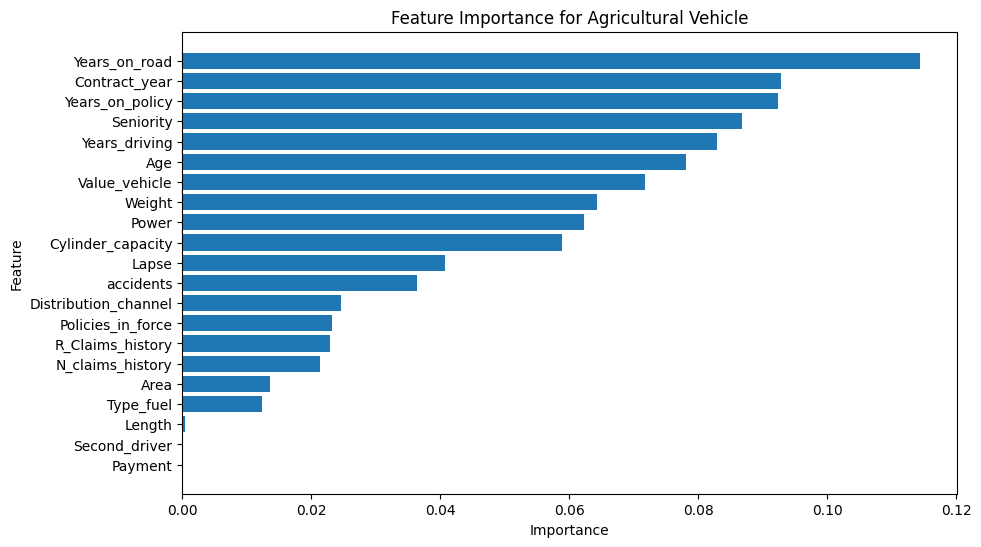
\includegraphics[width=\linewidth]{images/Agricultural Vehicle_feature_importance_random_forest.png}
        \caption{Agricultural Vehicles}
        \label{fig:subrandom4}
         \end{subfigure}
  \caption{Μοντέλο XGBoost που εκπαιδεύτηκε ξεχωριστά ανα κατηγορία}
  \label{fig:RandomForest_split_importance}
\end{figure}

\end{document}